%----------------------------------------------------------------------------------------
%	PACKAGES AND OTHER DOCUMENT CONFIGURATIONS
%----------------------------------------------------------------------------------------

\documentclass[landscape,a0paper,fontscale=0.5]{baposter} % Adjust the font scale/size here

\usepackage{graphicx} % Required for including images
\graphicspath{{figures/}} % Directory in which figures are stored

\usepackage{amsmath} % For typesetting math
\usepackage{amssymb} % Adds new symbols to be used in math mode

\usepackage{booktabs} % Top and bottom rules for tables
\usepackage{enumitem} % Used to reduce itemize/enumerate spacing
\usepackage{palatino} % Use the Palatino font
\usepackage[font=small,labelfont=bf]{caption} % Required for specifying captions to tables and figures

\usepackage{multicol} % Required for multiple columns
\setlength{\columnsep}{1.5em} % Slightly increase the space between columns
\setlength{\columnseprule}{0mm} % No horizontal rule between columns

\usepackage{tikz} % Required for flow chart
\usetikzlibrary{shapes,arrows} % Tikz libraries required for the flow chart in the template

\newcommand{\compresslist}{ % Define a command to reduce spacing within itemize/enumerate environments, this is used right after \begin{itemize} or \begin{enumerate}
\setlength{\itemsep}{1pt}
\setlength{\parskip}{0pt}
\setlength{\parsep}{0pt}
}

\definecolor{MRGGreen}{rgb}{0, 0.350, 0.200}

\newenvironment{ColFigure}
  {\par\medskip\noindent\minipage{\linewidth}}
  {\endminipage\par\medskip}


\begin{document}

\begin{poster}
{
headerborder=closed, % Adds a border around the header of content boxes
colspacing=1em, % Column spacing
bgColorOne=MRGGreen, % Background color for the gradient on the left side of the poster
bgColorTwo=MRGGreen, % Background color for the gradient on the right side of the poster
borderColor=MRGGreen, % Border color
headerColorOne=black, % Background color for the header in the content boxes (left side)
headerColorTwo=MRGGreen, % Background color for the header in the content boxes (right side)
headerFontColor=MRGGreen, % Text color for the header text in the content boxes
boxColorOne=white, % Background color of the content boxes
textborder=roundedleft, % Format of the border around content boxes, can be: none, bars, coils, triangles, rectangle, rounded, roundedsmall, roundedright or faded
eyecatcher=true, % Set to false for ignoring the left logo in the title and move the title left
headerheight=0.1\textheight, % Height of the header
headershape=roundedright, % Specify the rounded corner in the content box headers, can be: rectangle, small-rounded, roundedright, roundedleft or rounded
headerfont=\Large\bf\textsc, % Large, bold and sans serif font in the headers of content boxes
%textfont={\setlength{\parindent}{1.5em}}, % Uncomment for paragraph indentation
linewidth=2pt % Width of the border lines around content boxes
}
%----------------------------------------------------------------------------------------
%	TITLE SECTION 
%----------------------------------------------------------------------------------------
%
{
\includegraphics[height=4em]{graphics/logo.jpg}} % First university/lab logo on the left
{\bf\textsc{Unnecessarily Complicated Research Title}\vspace{0.5em}} % Poster title
{\textsc{\{ John Smith, James Smith and Jane Smith \} \hspace{12pt} University and Department Name}} % Author names and institution
{
\includegraphics[height=4em]{graphics/logo.jpg}} % Second university/lab logo on the right

%----------------------------------------------------------------------------------------
%	Introduction
%----------------------------------------------------------------------------------------

\headerbox{Introduction}{name=introduction,column=0,row=0,span=2}{
With increasing adoption of Bayesian inference to
pharmacometric(PMX) modeling, it has become evident that
high-performance computing(HPC) must be utilized for large-scale
models to be accessible, and inference framework based on Markov Chain
Monte Carlo(MCMC) must improve efficiency through multiple
channels. For example, probabilistic programming language Stan \cite{carpenter_stan_2017}
uses efficient samplers such as the No-U-Turn
Sampler(NUTS) \cite{hoffman_no-u-turn_2014}, and provide \texttt{\texttt{map\_rect}} functions
to parallelize expensive likelihood evaluation.

The scope of the work presented here is to improve Bayesian inference
efficiency of population models. The work is based on Torsten
\cite{Torsten}, a library of Stan functions that
simplifies PMX modeling and
extends the range of models that may be implemented. We address two
aspects of the efficiency problem. First, we propose a dynamic warmup
approach, as an alternative to current Stan's warmup where a fixed
number(default 1000) of iterations are performed. Second, we combine
the new warmup algorithm with existing within-chain parallelization
functionality of Torsten \cite{torsten_pmx_group} to formulate a \emph{multilevel} parallel method
that utilizes dynamic warmup \emph{and} within-chain parallelism to speed
up simulation.
}

%----------------------------------------------------------------------------------------
%	RESULTS 1
%----------------------------------------------------------------------------------------

\headerbox{Multilevel parallelization: cross-chain warmup + within-chain parallelization}{name=multilevel,column=2,span=2,row=0}{

\begin{multicols}{2}
\vspace{1em}
Combining cross-chain warmup and
within-chain parallelization, we are able to design a framework of
\emph{multilevel parallelism} for Bayesian inference of population
models. Orthogonal to the above warmup algorithm, \emph{within-chain}
parallelization implemented in Stan
and Torsten does not induce communication across chains but distributes a
heavy-lifting modeling task to mutiple processes in a single
chain. In Torsten this within-chain strategy focuses on solving ODEs
in population model.

Our multilevel framework has an upper and lower level of parallelization(Figure \ref{multilevel-diagram}). The upper
level handles the cross-chain warmup by running parallel chains and
updating metric and stepsize. Chains exchange
information only at the end of each window at this level. 

The lower level of within-chain parallelization occurs more
frequently: with every new set of parameter samples, NUTS updates the likelihhod
by solving the ODEs in the population model, and Torsten's group
solvers distribute the population to multiple processes, with each
processe handling one or several subjects' ODE systems.

\begin{center}
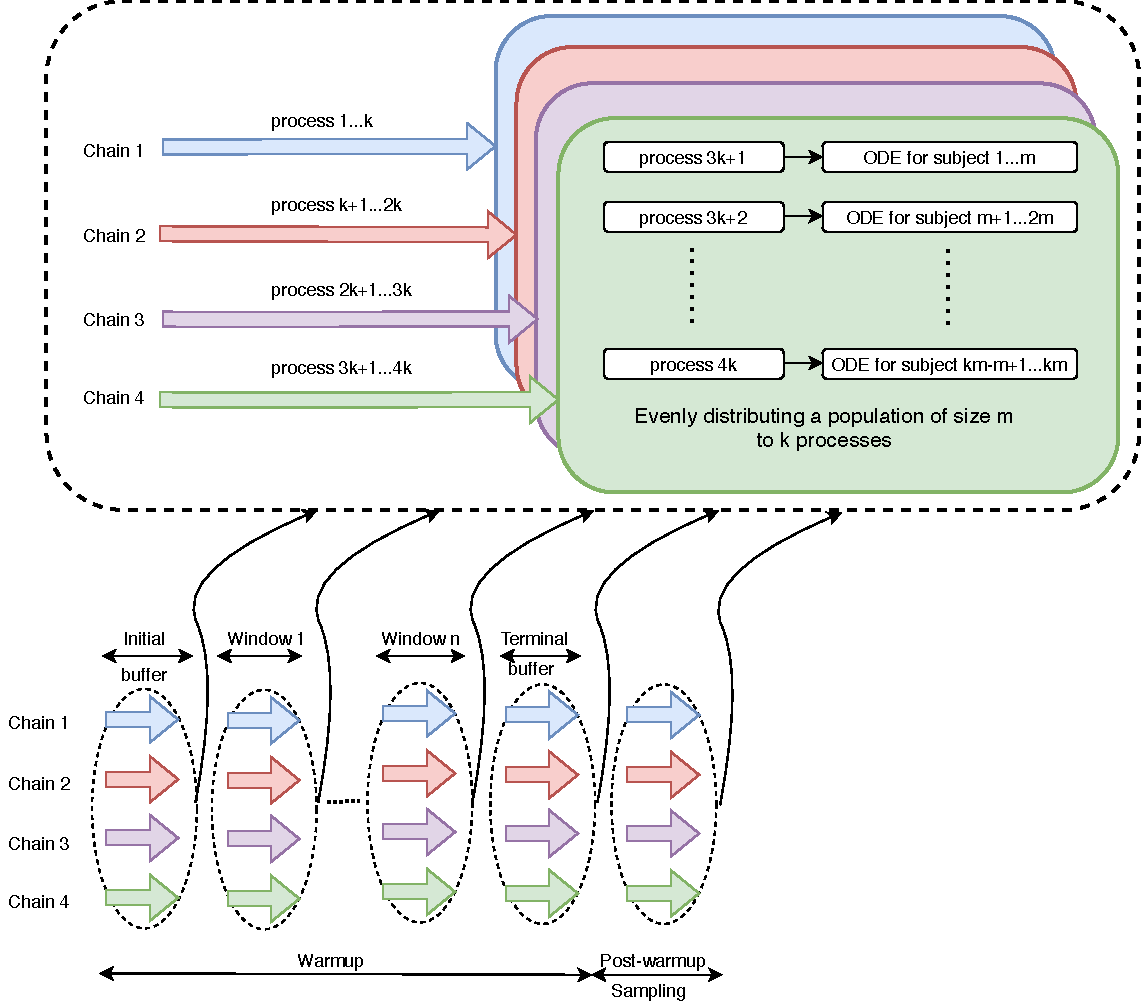
\includegraphics[width=\linewidth]{./figure/within_chain_parallel_diagram.pdf}
\captionof{figure}{Multilevel parallelism for ODE-based population models. A simplified version of Figure 1, the lower diagram shows the cross-chain warmup through multiple windows. In within-chain parallelization, as shown in the upper diagram, each chain has its own parameter samples(indicated by different colors), and dedicated processes for solving the population model. \label{multilevel-diagram}}
\end{center}

To demonstrate the above multilevel method, we apply it to a
time-to-event model for the time to the first grade 2+ peripheral neuropathy (PN)
event in patients treated with an antibody-drug conjugate (ADC)
delivering monomethyl auristatin E (MMAE). We call it
Time-To-PN(TTPN) model, and analyze data using a
simplified version of the model reported in
\cite{lu_time--event_2017}. We consider three treatment arms:
fauxlatuzumab vedotin 1.2, 1.8 and 2.4 mg/kg IV boluses q3w x 6 doses,
with 20 patients per treatment arm. In this model,
each patient's PK is described by an effective compartment model(one-compartment),
and PD by a linear model. The likelihood for time to first 2+ PN event
is described by a hazard function that depends on the concentration
effect through Weibull distribution. Two unknowns from
PK model and the cumulative hazard form a three-component
ODE system. Each evaluation of likelihood requires solving this
3-system for every patient. 

In Torsten's model, ODEs corresponding to the entire
population can be solved by a single call of \texttt{\texttt{pmx\_solve\_group\_rk45}} function. The three parameters of the
model are:
\begin{itemize}
\item \(k_{e0}\) in effective compartment model.
\item \(\alpha\) the coefficient of linear PD model.
\item \(\beta\) Weibull distribution scale parameter.
\end{itemize}

Similar to previous section, Figure shows performance of cross-chain and
regular runs based on target ESS = 400. Unlike in previous models, we
did not performe runs with multiple seed or target ESS to avoid long
computing time. One can make conclusion consistent with the other
models, that the cross-chain warmup reduce total run time without
compromising ESS.

\begin{center}
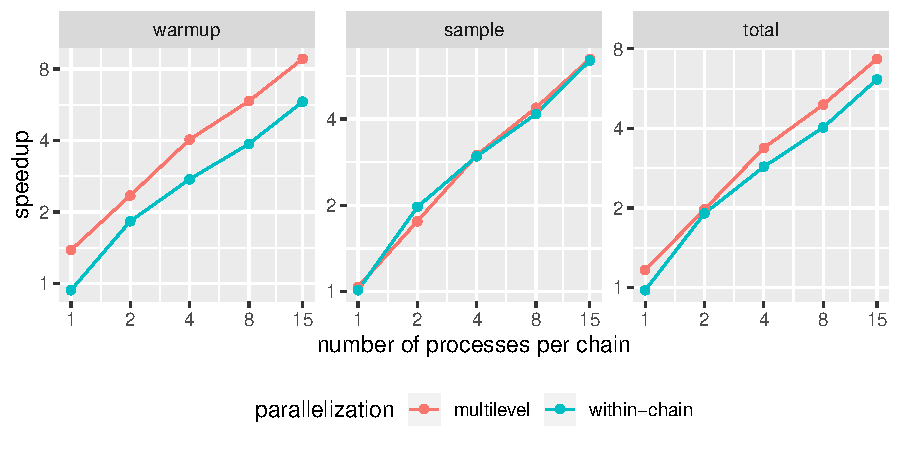
\includegraphics[width=\linewidth]{./figure/ttpn2_perf_benchmark.pdf}
\captionof{figure}{Multilevel scheme parallel performance based on TTPN model.}
\end{center}

Next, we apply multilevel method to TTPN model with a fixed target ESS
= 400, by running the model
with 4 chains using \(n_{\text{proc}} = 8, 16, 32, 60, 80\)
processes. Equivalently, there are
\(n_{\text{proc\_per\_chain}} = 2, 4, 8, 15, 20\)
processes per chain so that within-chain parallelization can be utilized.
With population size 60, each process handles solution of
\(n_{\text{id}} = 30, 15, 7, 4, 3\)
subjects' ODE system, respectively.

To show parallel scaling performance, we collect \texttt{\texttt{stanfit}} objects of the benchmark runs
and plot their wall time speedup against regular Stan runs. With all
runs having 1000 post-warmup sampling iterations, in
multilevel runs the number of warmup iterations is determinted at
runtime, while both within-chain parallel runs and regular Stan runs
have 1000 warmup iterations. Among 4 chains in a run, we use the
one with maximum total walltime(in seconds) as performance measure, as
in practice usually further model evaluation becomes accessible only
after all chains finish.

As shown in Figure \ref{cc-diagram}, both muiltilevel and
within-chai-only parallel runs exhibit good scaling up to 60
processes(15 processes per chain \(\times\) 4 chains)

\vspace{1em}
\end{multicols}

}

%----------------------------------------------------------------------------------------
%	REFERENCES
%----------------------------------------------------------------------------------------

\headerbox{References}{name=references,column=0,above=bottom}{

\renewcommand{\section}[2]{\vskip 0.05em} % Get rid of the default "References" section title
\nocite{*} % Insert publications even if they are not cited in the poster
\small{ % Reduce the font size in this block
\bibliographystyle{siam}
\bibliography{sample} % Use sample.bib as the bibliography file
}}

%----------------------------------------------------------------------------------------
%	FUTURE RESEARCH
%----------------------------------------------------------------------------------------

\headerbox{Future Research}{name=futureresearch,column=1,span=2,aligned=references,above=bottom}{ % This block is as tall as the references block

\begin{multicols}{2}
Integer sed lectus vel mauris euismod suscipit. Praesent a est a est ultricies pellentesque. Donec tincidunt, nunc in feugiat varius, lectus lectus auctor lorem, egestas molestie risus erat ut nibh.

Maecenas viverra ligula a risus blandit vel tincidunt est adipiscing. Suspendisse mollis iaculis sem, in \emph{imperdiet} orci porta vitae. Quisque id dui sed ante sollicitudin sagittis.
\end{multicols}
}

%----------------------------------------------------------------------------------------
%	CONTACT INFORMATION
%----------------------------------------------------------------------------------------

\headerbox{Contact Information}{name=contact,column=3,aligned=references,above=bottom}{ % This block is as tall as the references block

\begin{description}\compresslist
\item[Web] www.university.edu/smithlab
\item[Email] john@smith.com
\item[Phone] +1 (000) 111 1111
\end{description}
}

%----------------------------------------------------------------------------------------
%	CONCLUSION
%----------------------------------------------------------------------------------------

\headerbox{Conclusion}{name=conclusion,column=2,span=2,row=0,below=results,above=references}{

\begin{multicols}{2}

\tikzstyle{decision} = [diamond, draw, fill=blue!20, text width=4.5em, text badly centered, node distance=2cm, inner sep=0pt]
\tikzstyle{block} = [rectangle, draw, fill=blue!20, text width=5em, text centered, rounded corners, minimum height=4em]
\tikzstyle{line} = [draw, -latex']
\tikzstyle{cloud} = [draw, ellipse, fill=red!20, node distance=3cm, minimum height=2em]

\begin{tikzpicture}[node distance = 2cm, auto]
\node [block] (init) {Initialize Model};
\node [cloud, left of=init] (Start) {Start};
\node [cloud, right of=init] (Start2) {Start Two};
\node [block, below of=init] (init2) {Initialize Two};
\node [decision, below of=init2] (End) {End};
\path [line] (init) -- (init2);
\path [line] (init2) -- (End);
\path [line, dashed] (Start) -- (init);
\path [line, dashed] (Start2) -- (init);
\path [line, dashed] (Start2) |- (init2);
\end{tikzpicture}

%------------------------------------------------

\begin{itemize}\compresslist
\item Pellentesque eget orci eros. Fusce ultricies, tellus et pellentesque fringilla, ante massa luctus libero, quis tristique purus urna nec nibh. Phasellus fermentum rutrum elementum. Nam quis justo lectus.
\item Vestibulum sem ante, hendrerit a gravida ac, blandit quis magna.
\item Donec sem metus, facilisis at condimentum eget, vehicula ut massa. Morbi consequat, diam sed convallis tincidunt, arcu nunc.
\item Nunc at convallis urna. isus ante. Pellentesque condimentum dui. Etiam sagittis purus non tellus tempor volutpat. Donec et dui non massa tristique adipiscing.
\end{itemize}

\end{multicols}
}

%----------------------------------------------------------------------------------------
%	MATERIALS AND METHODS
%----------------------------------------------------------------------------------------

\headerbox{Cross-chain warmup}{name=warmup,column=0,span=2,below=introduction,bottomaligned=conclusion}{ % This block's bottom aligns with the bottom of the conclusion block
\begin{multicols}{2}
\vspace{1em}
The standard practice of Stan is to perform a fixed number of warmup
iterations. With this practice, the efficacy of the warmup is unknown
\emph{a priori} and often warmup is unncessarily long as user oversubscribe warmup iterations.
The proposed warmup algorithm tries to avoid this by checking potential scale reduction
coefficients (\(\hat{R}\)) and effective sample sizes (ESS)
\cite{vehtari_rank-normalization_2019} . Specifically, for warmup we
propose
\begin{ColFigure}
 \centering
 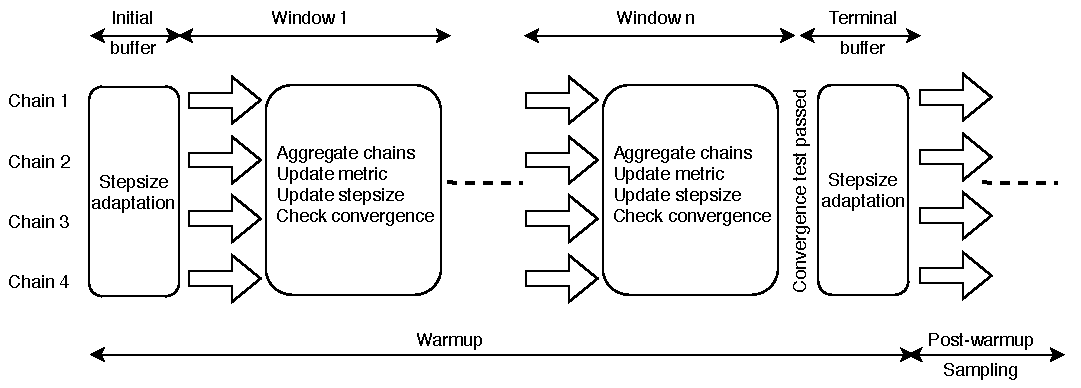
\includegraphics[width=\linewidth]{figure/cross_chain_diagram.pdf}
 \captionof{figure}{my caption of the figure}
\end{ColFigure}

\begin{enumerate}
\item Given a fixed window size \(w\)(default 100 iterations), the sampler iterates during warmup with stepsize adapted as in regular warmup runs.
\item At the end of a window, joint posterior probability from all the
  chains are aggregated and used to calculate corresponding \(\hat{R}\) and ESS. 
For example, with default window size \(w=100\), when warmup reaches iteration 300, we calculate
\(\hat{R}^i\) and \(\text{ESS}^i\) for \(i=1, 2, 3\), so that
\(\hat{R}^1\) and \(\text{ESS}^1\) are based on warmup iteration 1 to 300,
\(\hat{R}^2\) and \(\text{ESS}^2\) are based on warmup iteration 101 to 300,
and
\(\hat{R}^3\) and \(\text{ESS}^3\) are based on warmup iteration 201 to 300.

\item At the end of window \(n\), with predefined target value
  \(\hat{R}^{0}\) and ESS\(^{0}\), from \({1, \dots, n}\),  we select
  \(j\) with maximum 
$\text{ESS}^j$,
and a new metric is calculated by aggregating samples from
corresponding windows.
If, in addition, \(j\) satisfies $\hat{R}^j < \hat{R}^0$ and $\text{ESS}^j > \text{ESS}^0$,
the warmup is considered complete((\emph{converges}). Otherwise warmup continues until
the end of the next window and step 2-3 are repeated.
\end{enumerate}
Unlike current warmup scheme, the above proposal requires
communication among the chains, hence we call it \emph{cross-chain warmup}.

In benchmark, the above warmup scheme is compared against standard Stan warmup(1000
iterations) on several models for their
\begin{ColFigure}
\centering
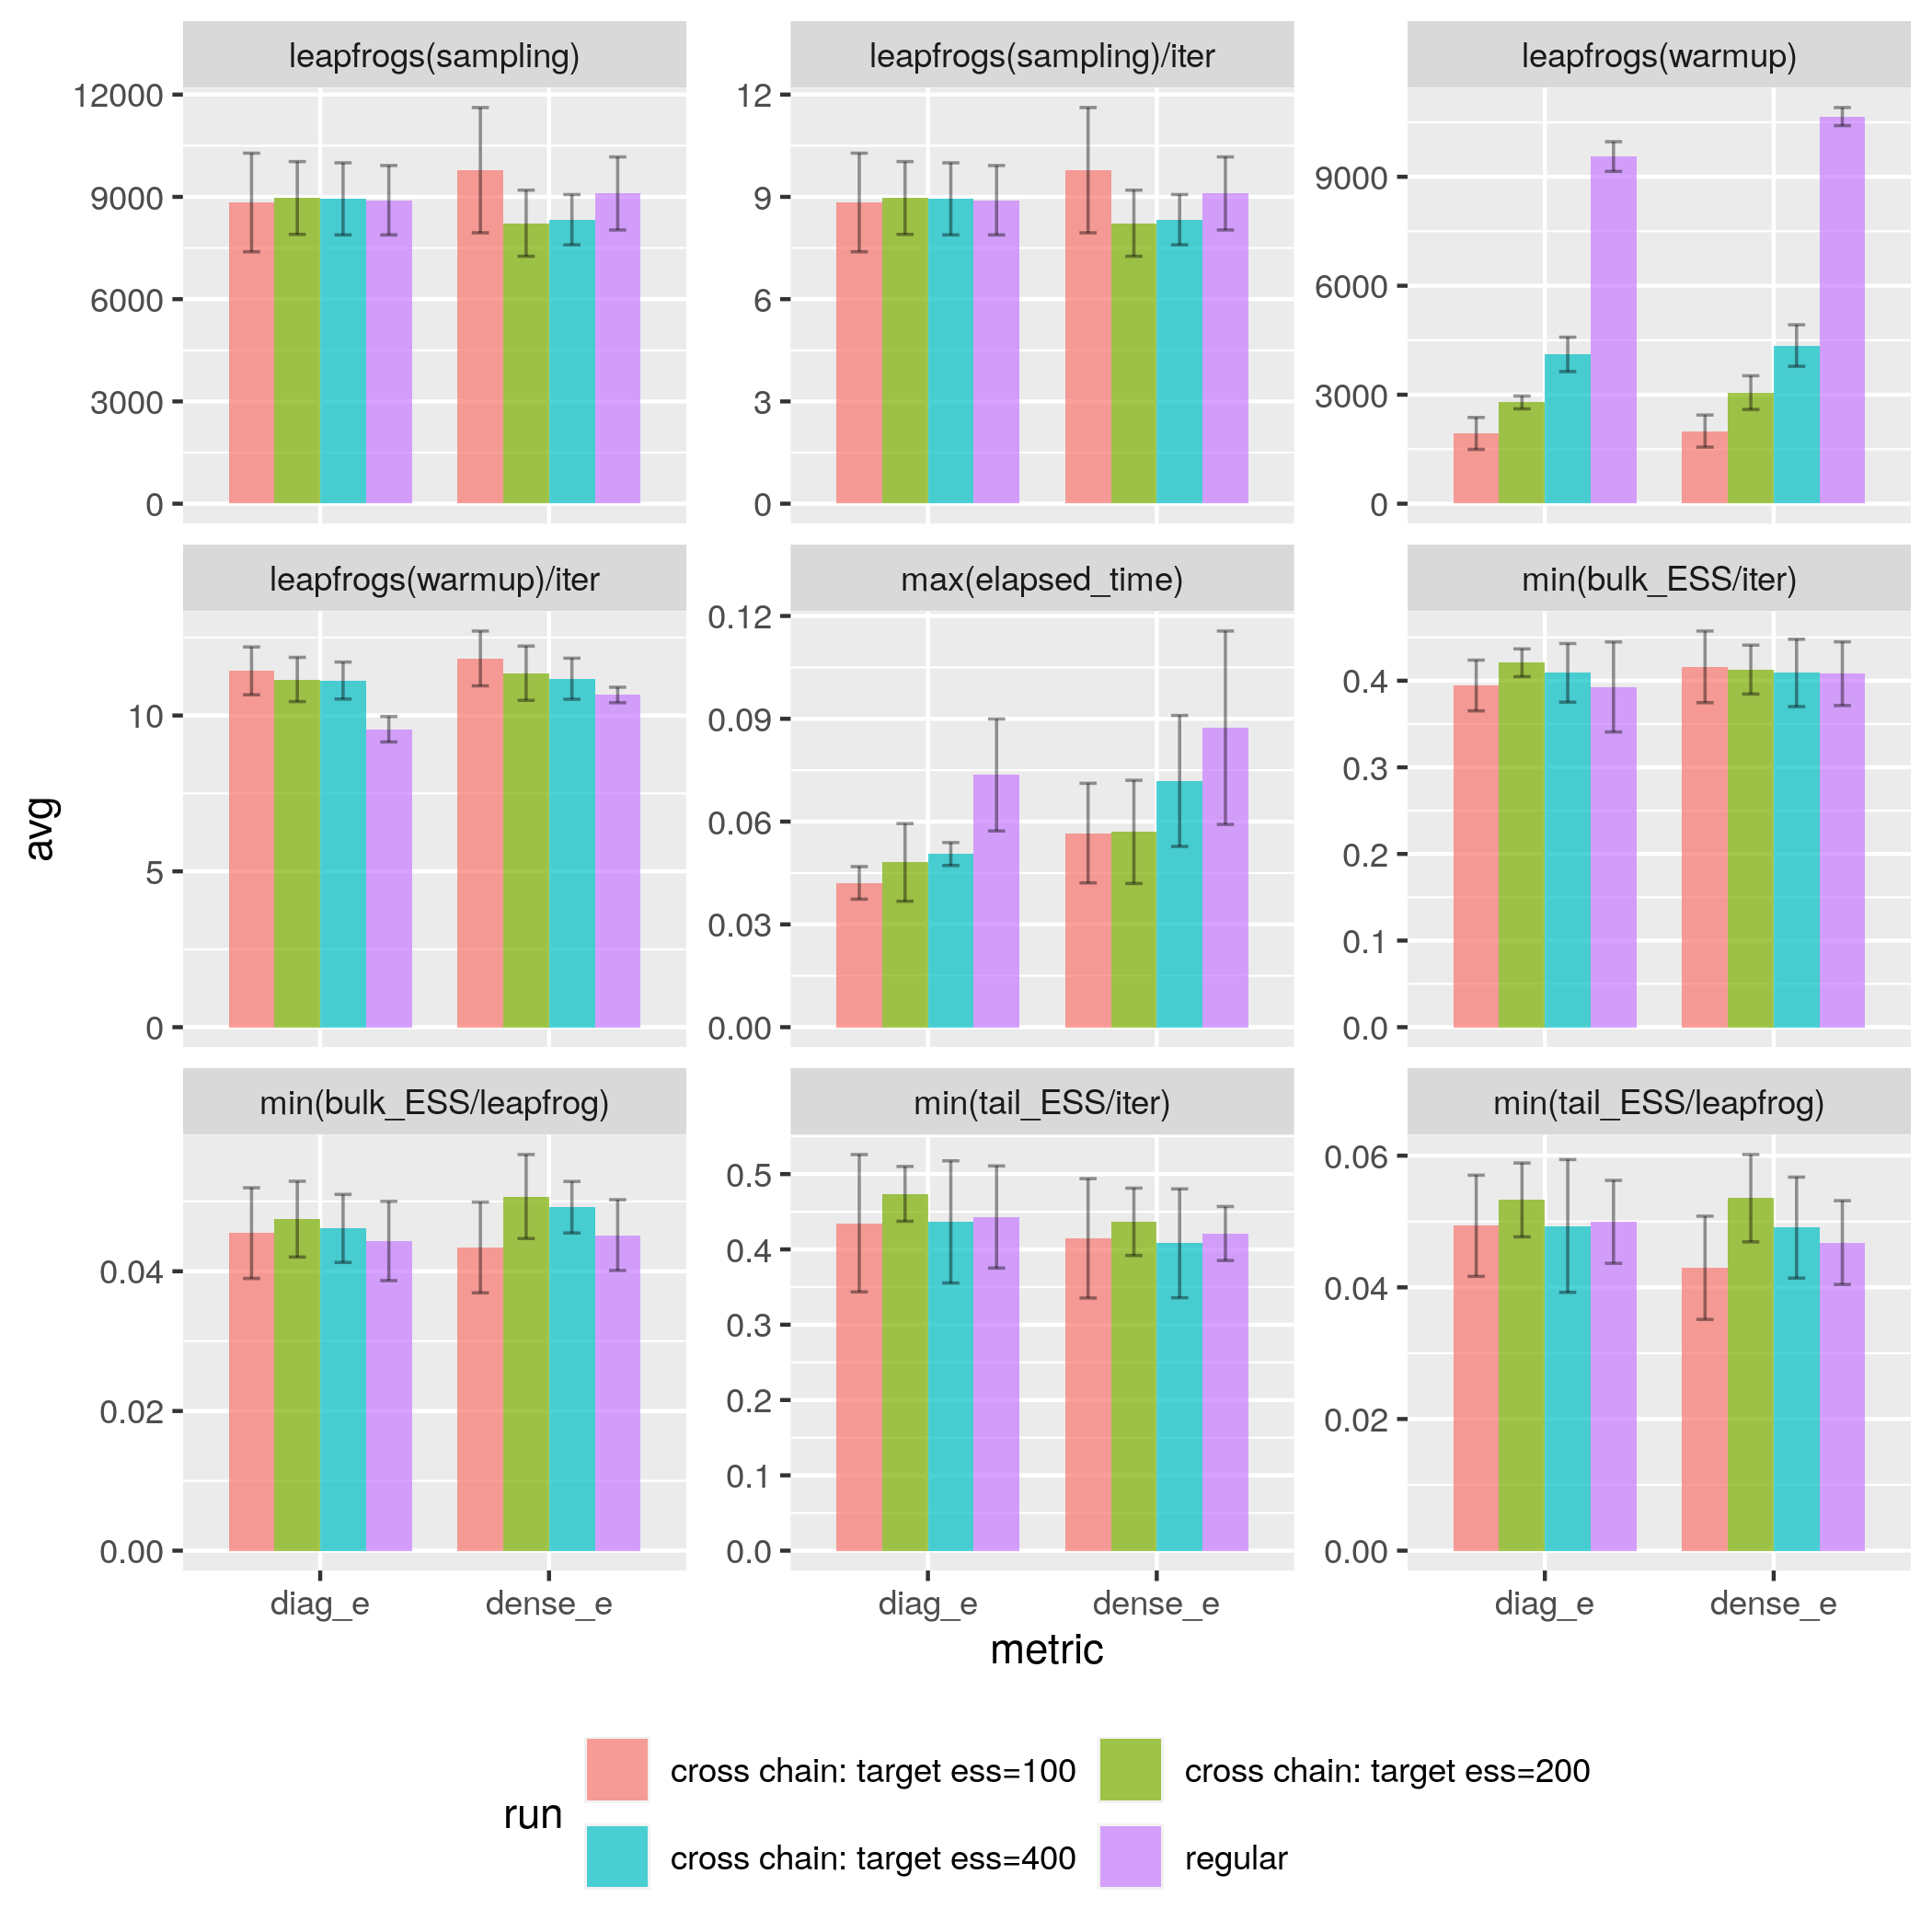
\includegraphics[width=0.8\linewidth]{./figure/cross_chain_ess_effect_eight_schools.png}
\captionof{figure}{Cross-chain warmup performance comparison: eight schools model}
\end{ColFigure}

\begin{ColFigure}
\centering
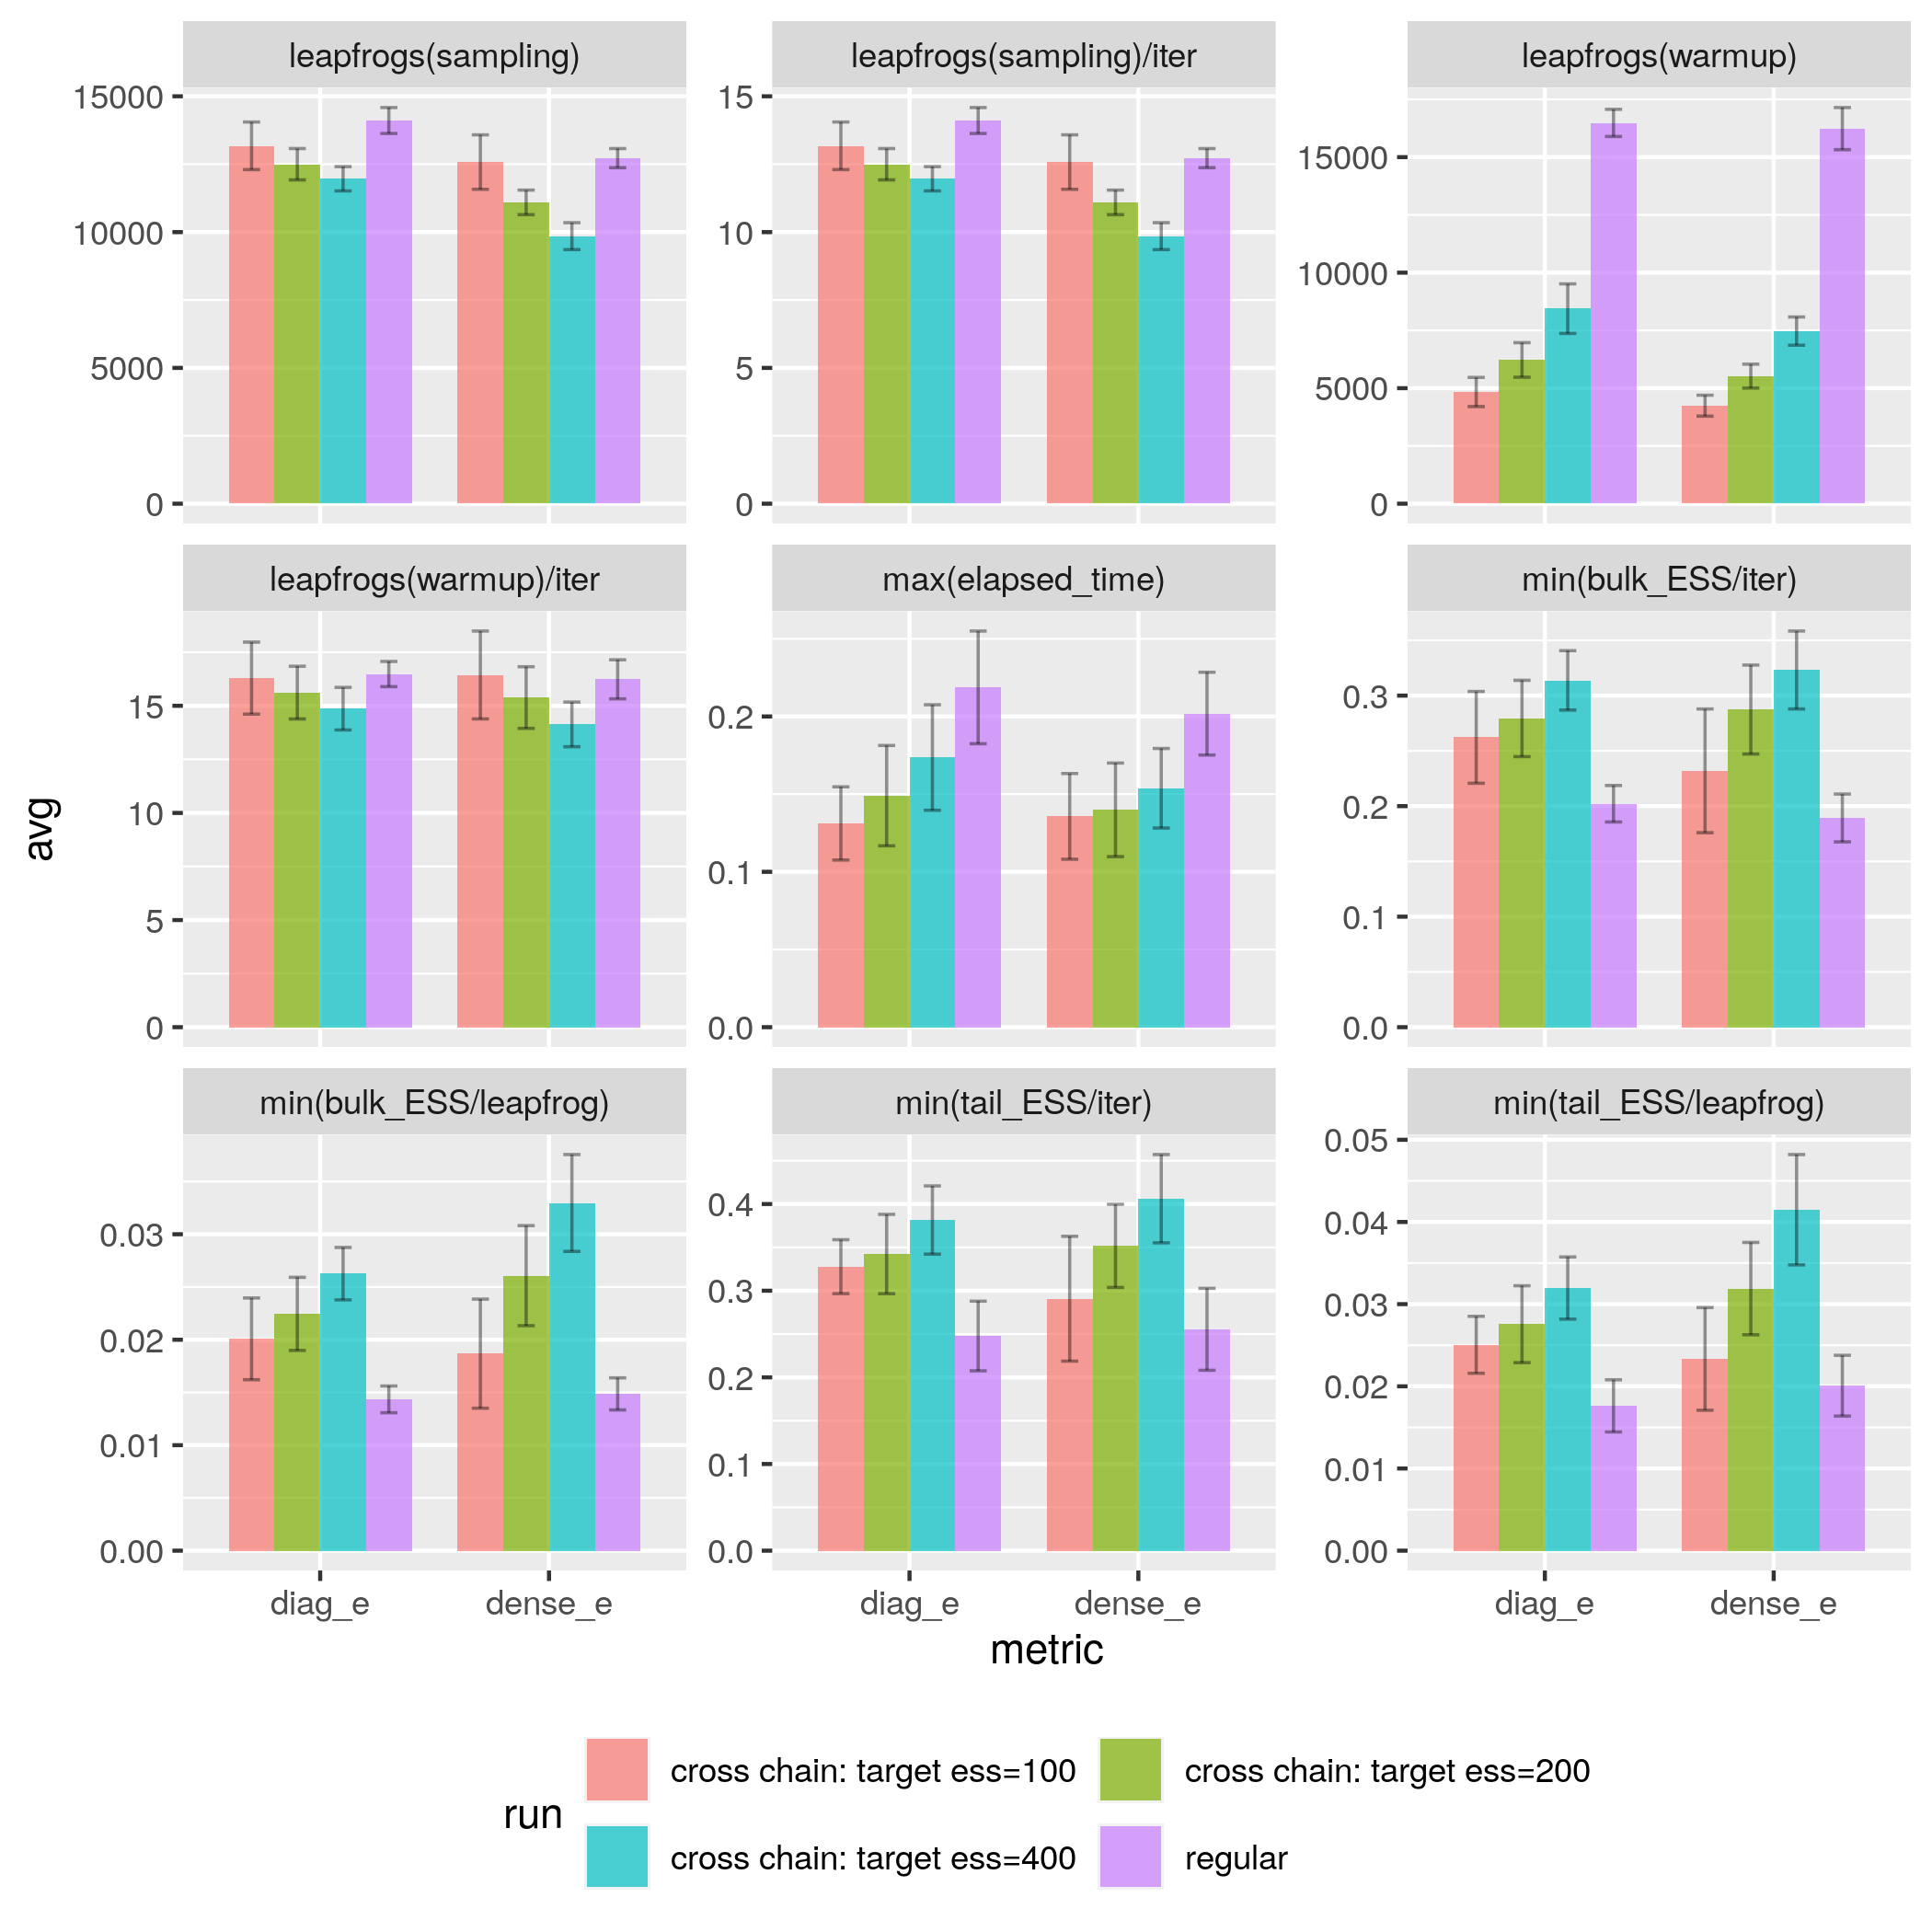
\includegraphics[width=0.8\linewidth]{./figure/cross_chain_ess_effect_sblrc-blr.png}
\caption{Cross-chain warmup performance comparison: garch-garch11 model}
\end{ColFigure}

\begin{ColFigure}
\centering
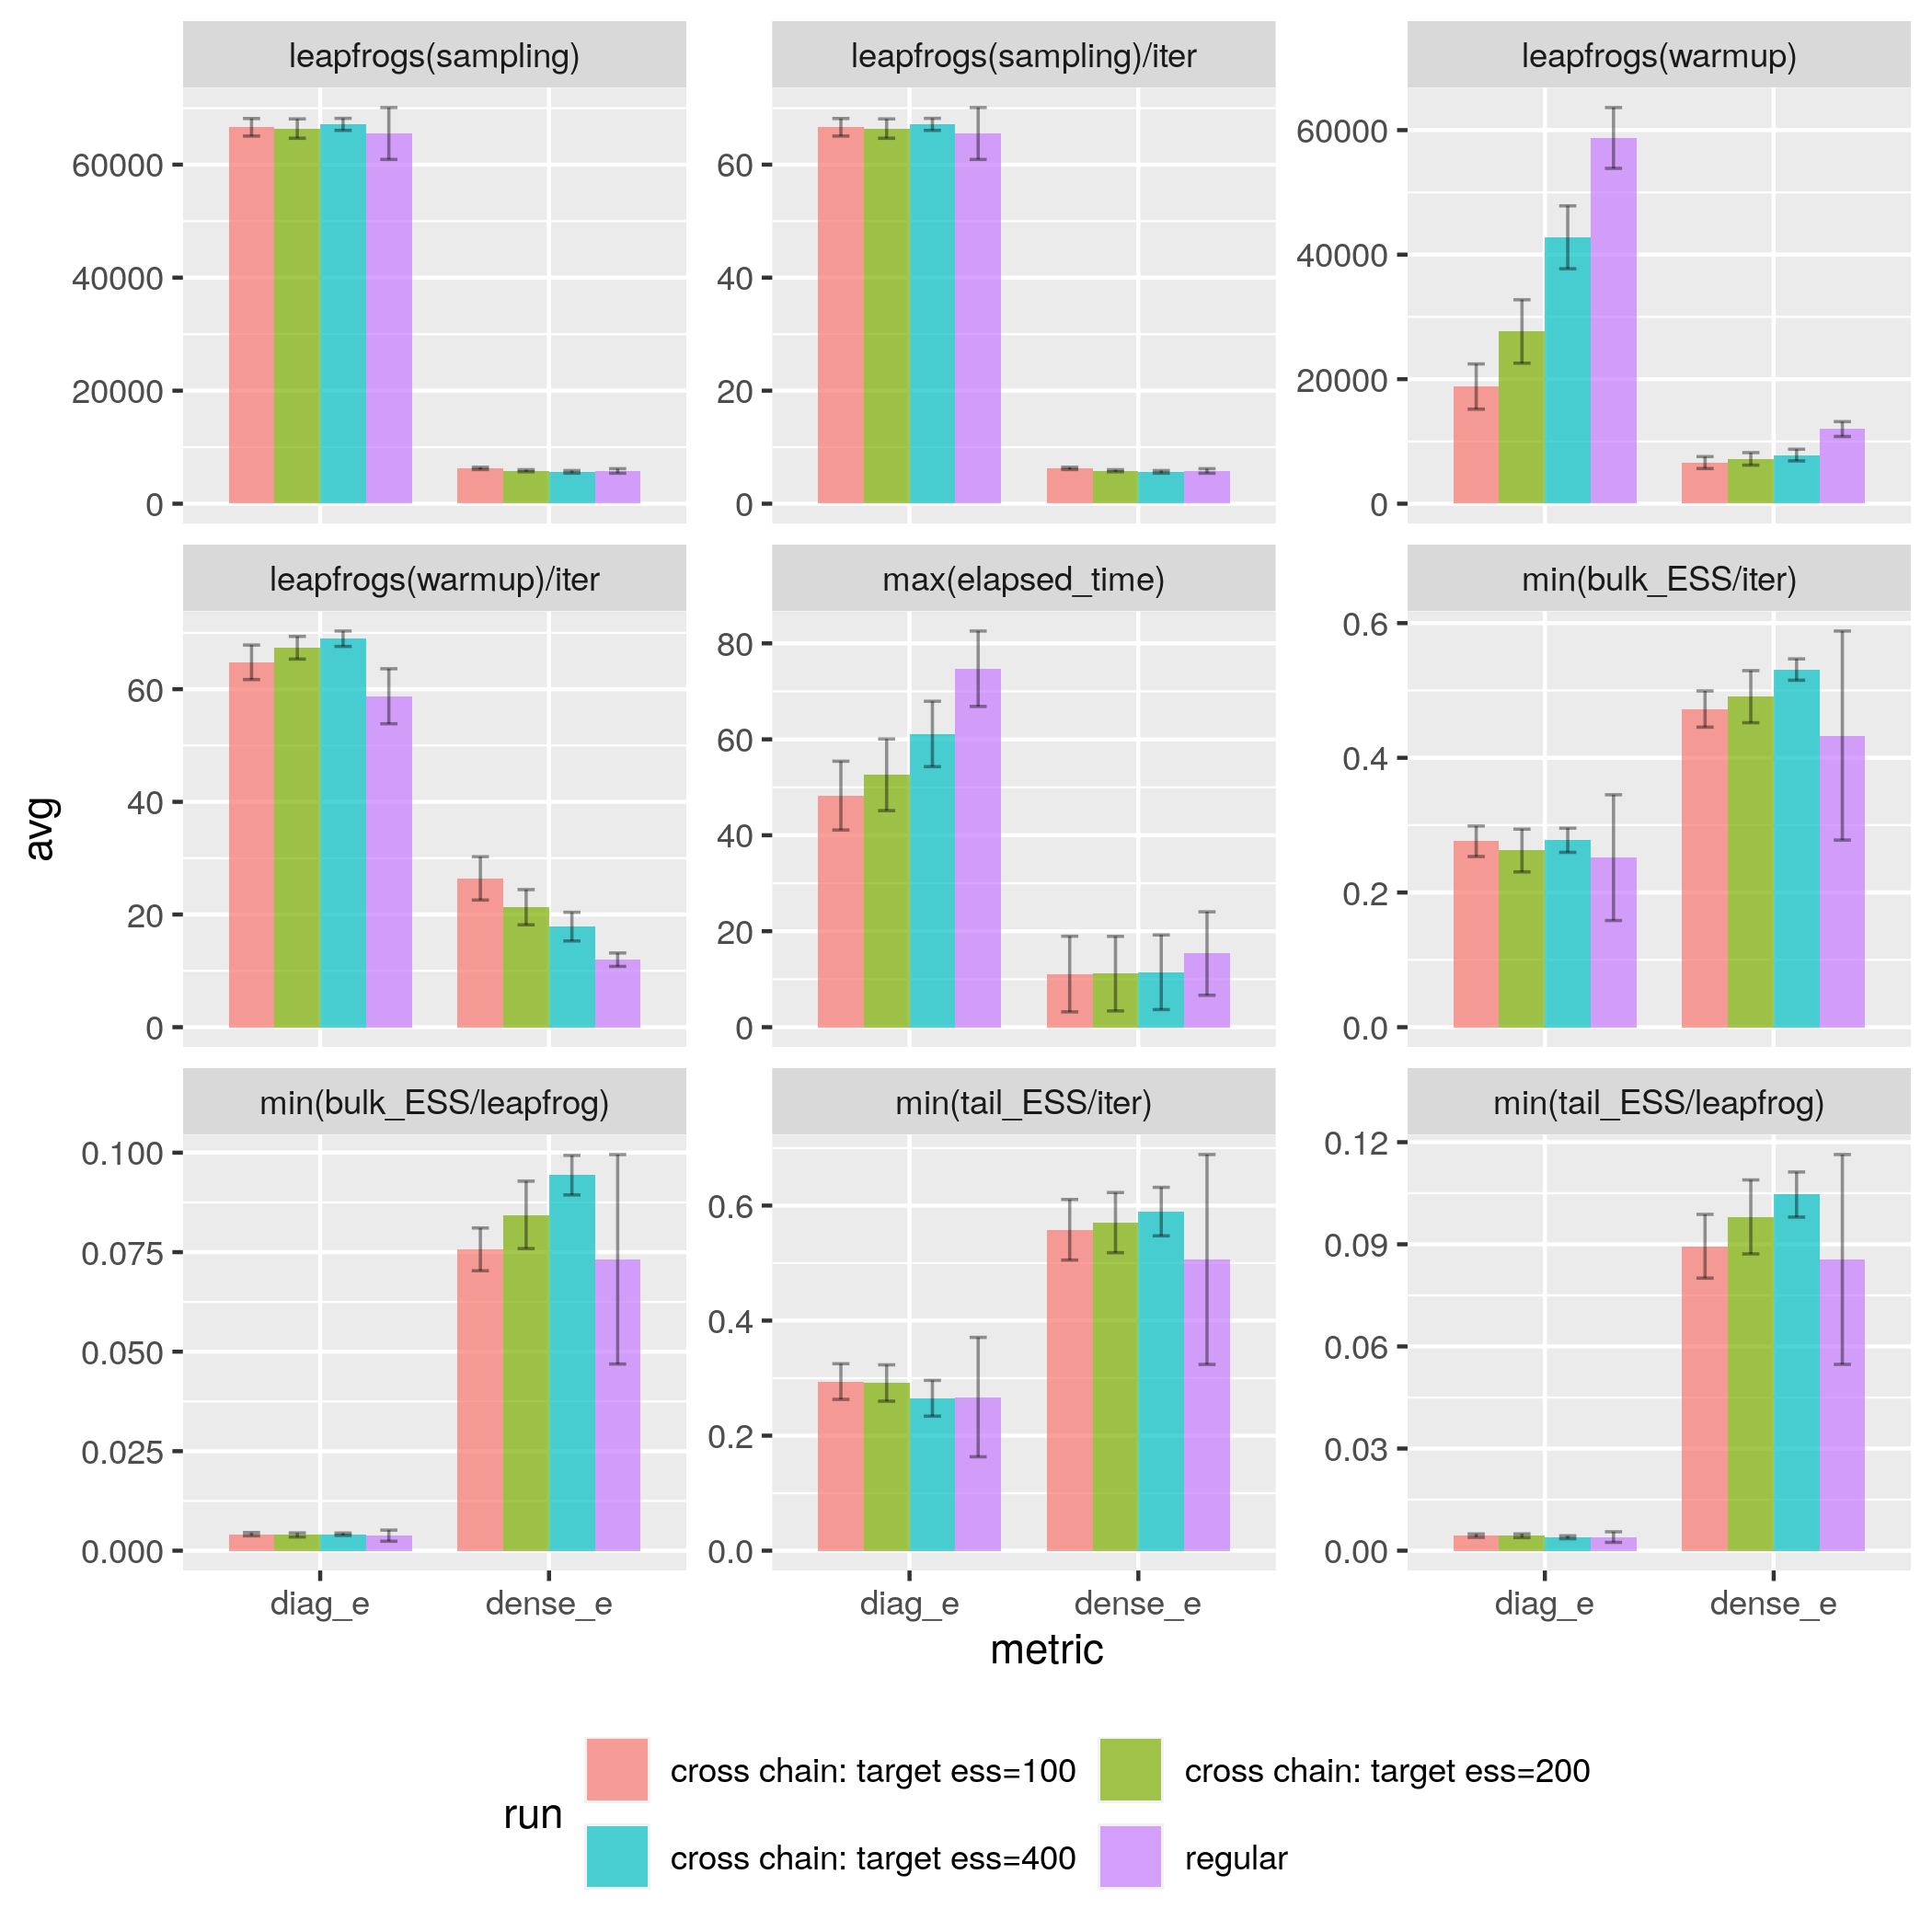
\includegraphics[width=0.8\linewidth]{./figure/cross_chain_ess_effect_sir.png}
\caption{Cross-chain warmup performance comparison: SIR model}
\end{ColFigure}

\begin{center}
\begin{tabular}{l}
\hline
total number of leapfrog integration steps in warmup \\
total number of leapfrog integration steps in sampling \\
number of leapfrog integration steps in per each warmup iteration \\
number of leapfrog integration steps in per each sampling iteration \\
minimum ESS\(_{\text{bulk}}\) per iteration \\
minimum ESS\(_{\text{tail}}\) per iteration \\
minimum ESS\(_{\text{bulk}}\) per leapfrog step \\
minimum ESS\(_{\text{tail}}\) per leapfrog step \\
maximum wall time
\hline
\end{tabular}
\end{center}
Each setup is run with 10 PRNG seeds and the quantities' average(barplot)
and standard deviation(error bar) are shown. All wall time are in seconds.

% \begin{ColFigure}
% \centering
% 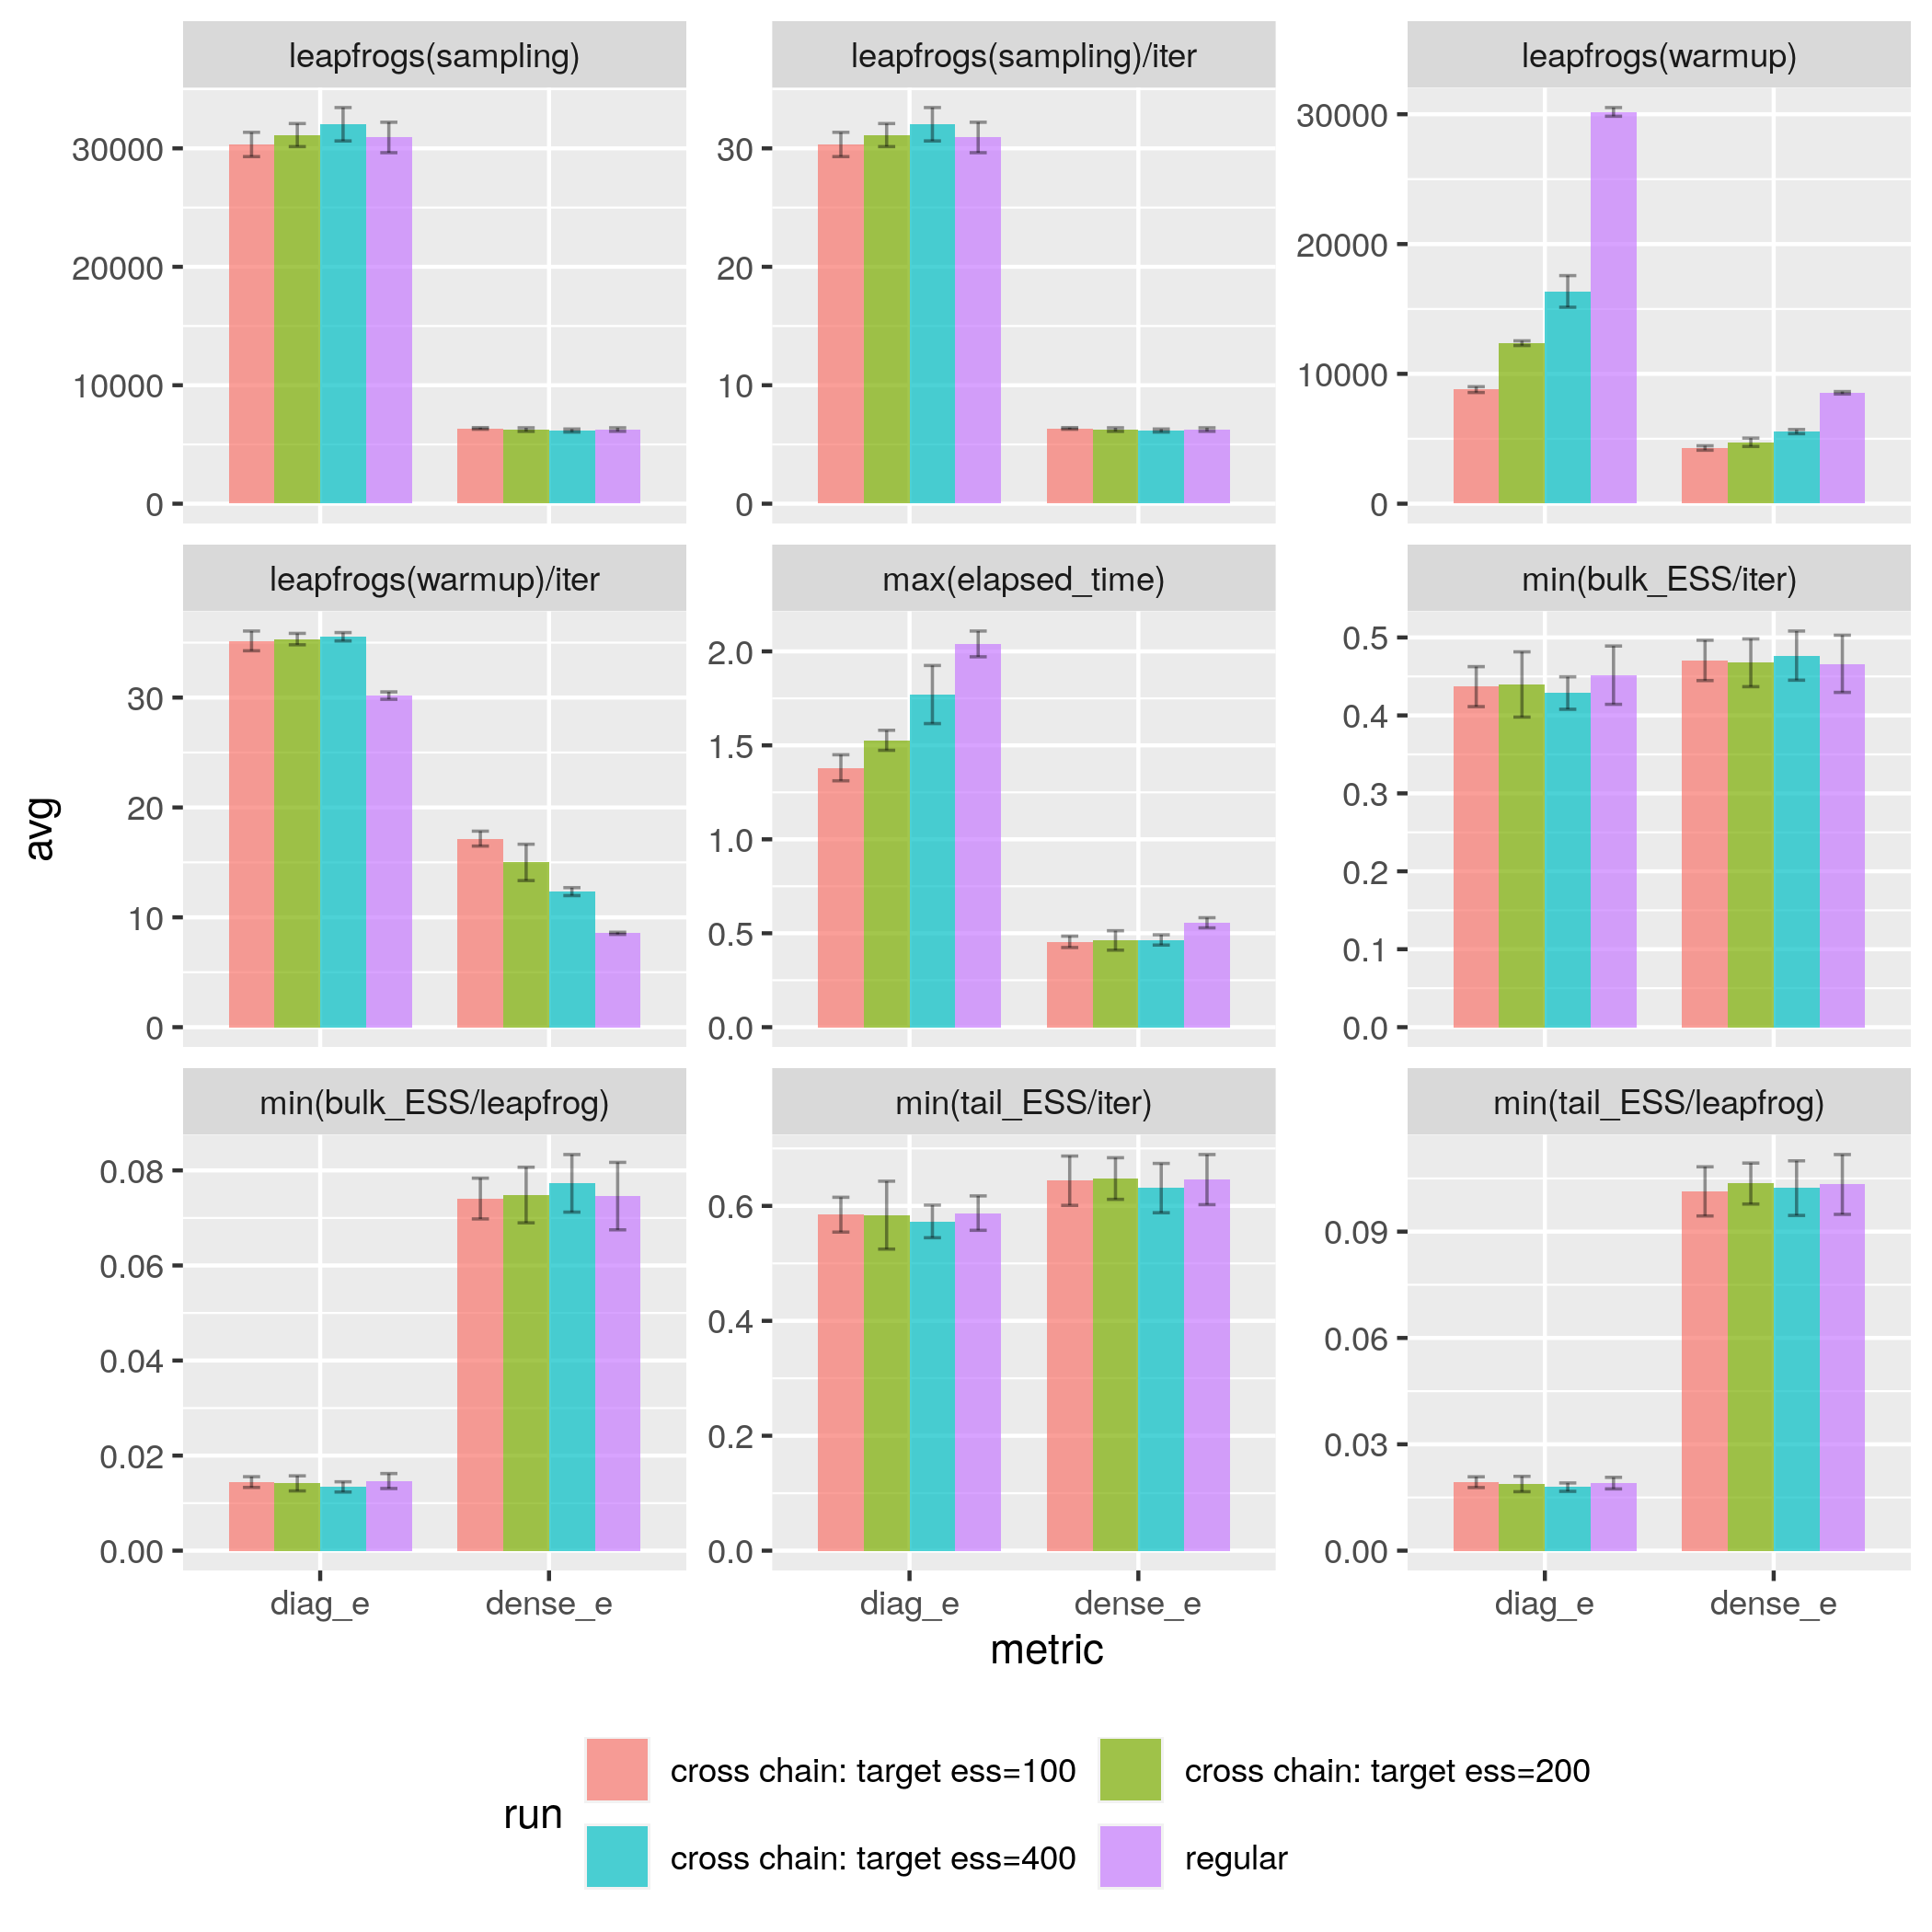
\includegraphics[width=0.7\linewidth]{./figure/cross_chain_ess_effect_arK.png}
% \caption{Cross-chain warmup performance comparison: arK model}
% \end{ColFigure}


% \begin{ColFigure}
% \centering
% 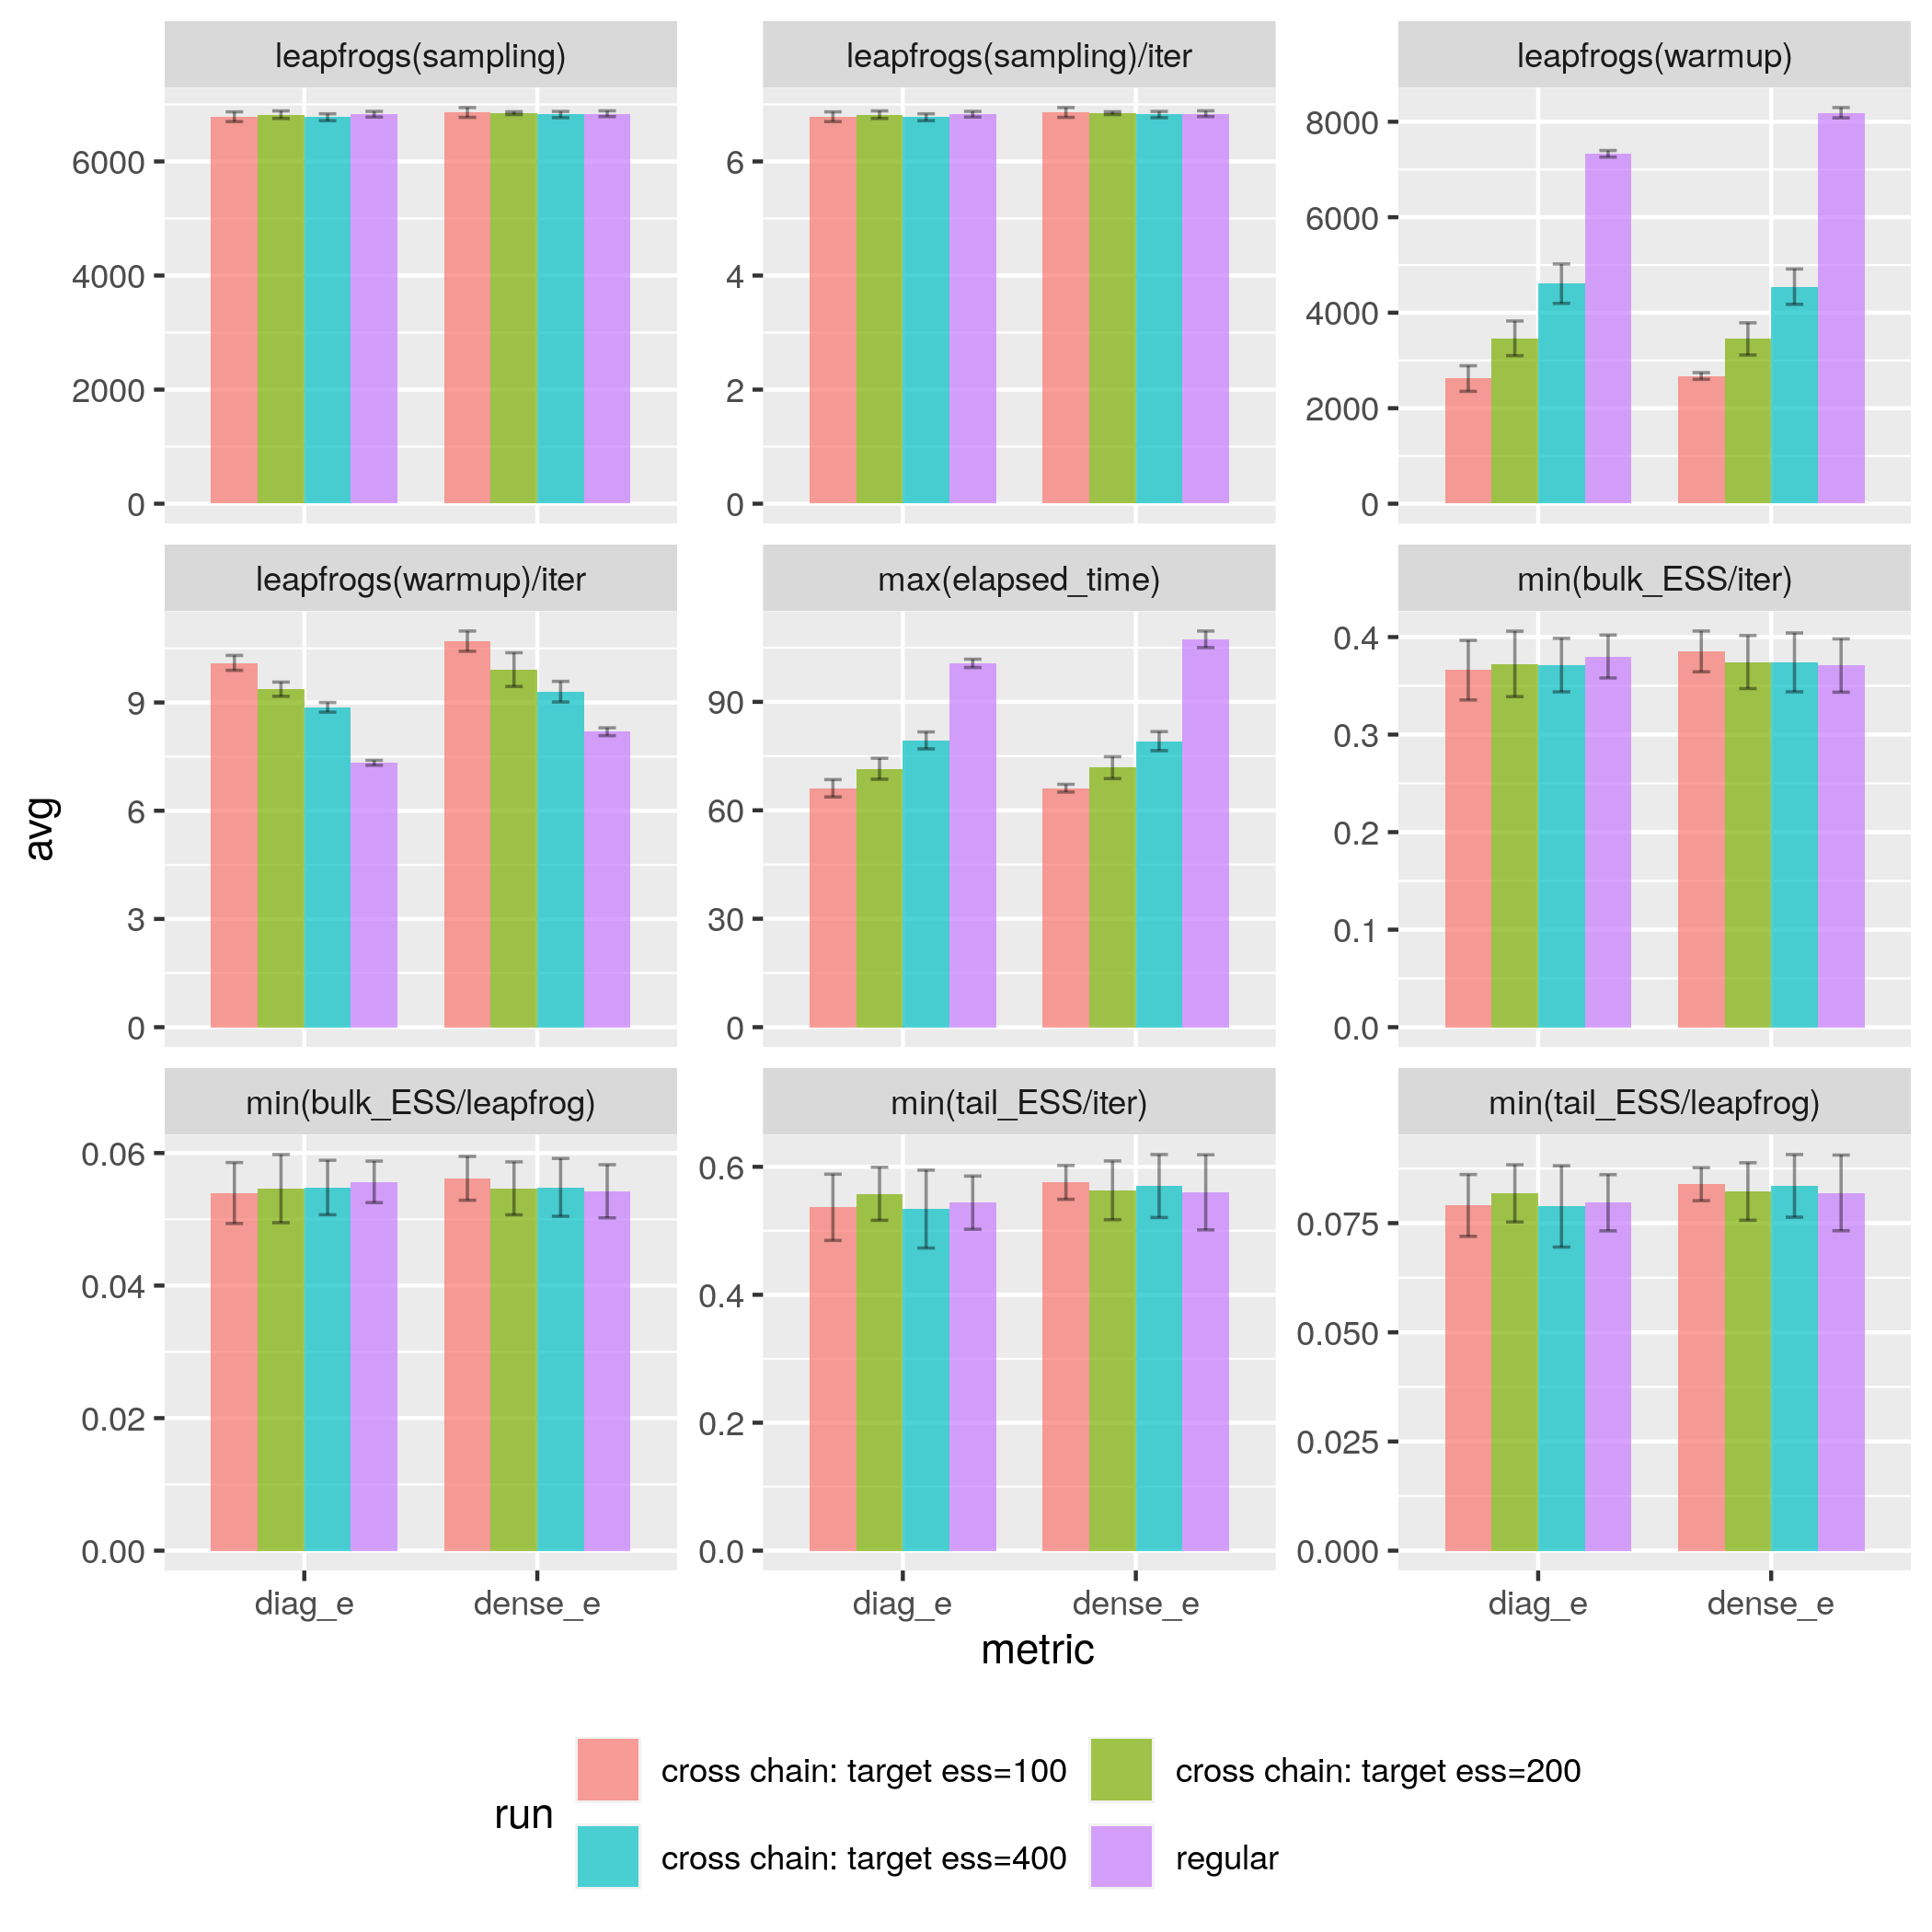
\includegraphics[width=0.7\linewidth]{./figure/cross_chain_ess_effect_chem.png}
% \caption{Cross-chain warmup performance comparison: chemical reaction model}
% \end{ColFigure}

\end{multicols}

% \begin{enumerate}
% \item Given a fixed window size \(w\)(default 100) and initial buffer size(default 75), the sampler iterates during warmup with stepsize adapted as in regular warmup runs.
% \item At the end of a window, we aggregate the joint posterior probability \texttt{lp\_\_} from all the chains and calculate corresponding \(\hat{R}\) as well as ESS. 
% Specifically, when the warmup reaches the last iteration of window
% \(n\), we calculate \(\hat{R}^i\) and \(\text{ESS}^i\), \(i=1\dots,n\). The
% superscript \(i\) indicates that the quantity is calculated based on
% \texttt{lp\_\_} aggregated from all the chains, using the iterations from
% window \(i\), \(i+1\), \dots{}, \(n\). For example, with default window
% size \(w=100\), when warmup reaches iteration 300, we calculate
% \(\hat{R}^i\) and \(\text{ESS}^i\) for \(i=1, 2, 3\), so that

% \(\hat{R}^1\) and \(\text{ESS}^1\) are based on warmup iteration 1 to 300;

% \(\hat{R}^2\) and \(\text{ESS}^2\) are based on warmup iteration 101 to 300;

% \(\hat{R}^3\) and \(\text{ESS}^3\) are based on warmup iteration 201 to 300.

% \item At the end of window \(n\), with predefined target value \(\hat{R}^{0}\) and ESS\(^{0}\), from \({1, \dots, n}\),  we select \(j\) such that
% \begin{equation}
% \text{ESS}^j > \text{ESS}^i,\quad \forall i\neq j, \quad 1\le i\le n.
% \end{equation}
% Namely, we select \(j\) so that it has the maximum ESS. A new metric
% is calculated by aggregating samples from

% \begin{equation*}   
%    \text{window } j, \text{window } j+1, ..., \text{window } n
% \end{equation*}
% from all the chains, and a new stepsize is calculated by taking geometric mean
% of chain stepsizes. The new metric and stepsize are used in future iterations for all the chains.
% If, in addition, \(j\) satisfies
% \begin{equation}
% \begin{aligned}
% \hat{R}^j < \hat{R}^0,\\
% \text{ESS}^j > \text{ESS}^0,
% \end{aligned}
% \end{equation}
% the warmup is considered complete(\emph{converges}). Otherwise warmup continues until
% the end of the next window and step 2-3 are repeated.
% \item After convergences, the warmup
% continues into terminal buffer(50 iterations by default). As in
% standard Stan warmup, in this buffer the metric is no longer
% updated while stepsize is further adapted.
% \end{enumerate}

% Unlike current warmup scheme, the above proposal requires
% communication among the chains, hence we call it \emph{cross-chain warmup}.
% The implementation is based on Torsten's parallel setup using Message
% Passing Interface (MPI). In
% a cross-chain warmup run, all chains move forward independently except
% at the end of a window, where samples are aggregated from the chains
% to calculate \(\hat{R}^i\) and ESS\(^i\) and new metric and stepsize are
% distributed to the chains.
% After warmup the sampler moves into independent post-warmup sampling stage
% with no more cross-chain communications.


% \begin{verbatim}
% \subsection*{Performance evaluation}
% \end{verbatim}
% We compare the two warmup schemes by running several models
% from \href{https://github.com/MansMeg/posteriordb}{posteriordb} and \href{https://github.com/metrumresearchgroup/Torsten/tree/master/example-models}{Torsten} repo. For each model, we compare the
% effect of warmup on 
% \begin{itemize}
% \item total number of leapfrog integration steps in warmup
% \item total number of leapfrog integration steps in sampling
% \item number of leapfrog integration steps in per each warmup iteration
% \item number of leapfrog integration steps in per each sampling iteration
% \item minimum ESS\(_{\text{bulk}}\) per iteration
% \item minimum ESS\(_{\text{tail}}\) per iteration
% \item minimum ESS\(_{\text{bulk}}\) per leapfrog step
% \item minimum ESS\(_{\text{tail}}\) per leapfrog step
% \item maximum wall time
% \end{itemize}

% We run each model runs with 10 random seeds 
% \begin{verbatim}
% seed <- seq(8235121, 8235130)
% \end{verbatim}
% and plot the above
% quantities' the average(barplot)
% and standard deviation(error bar).

% For profiling cross-chain performance of a particular model, we compare
% fit results from different target ESS as well as regular runs(4 chains
% with 1000 warmup iterations in each chain). All wall time in this report are measured in seconds.

% \begin{figure}[htbp]
% \centering
% 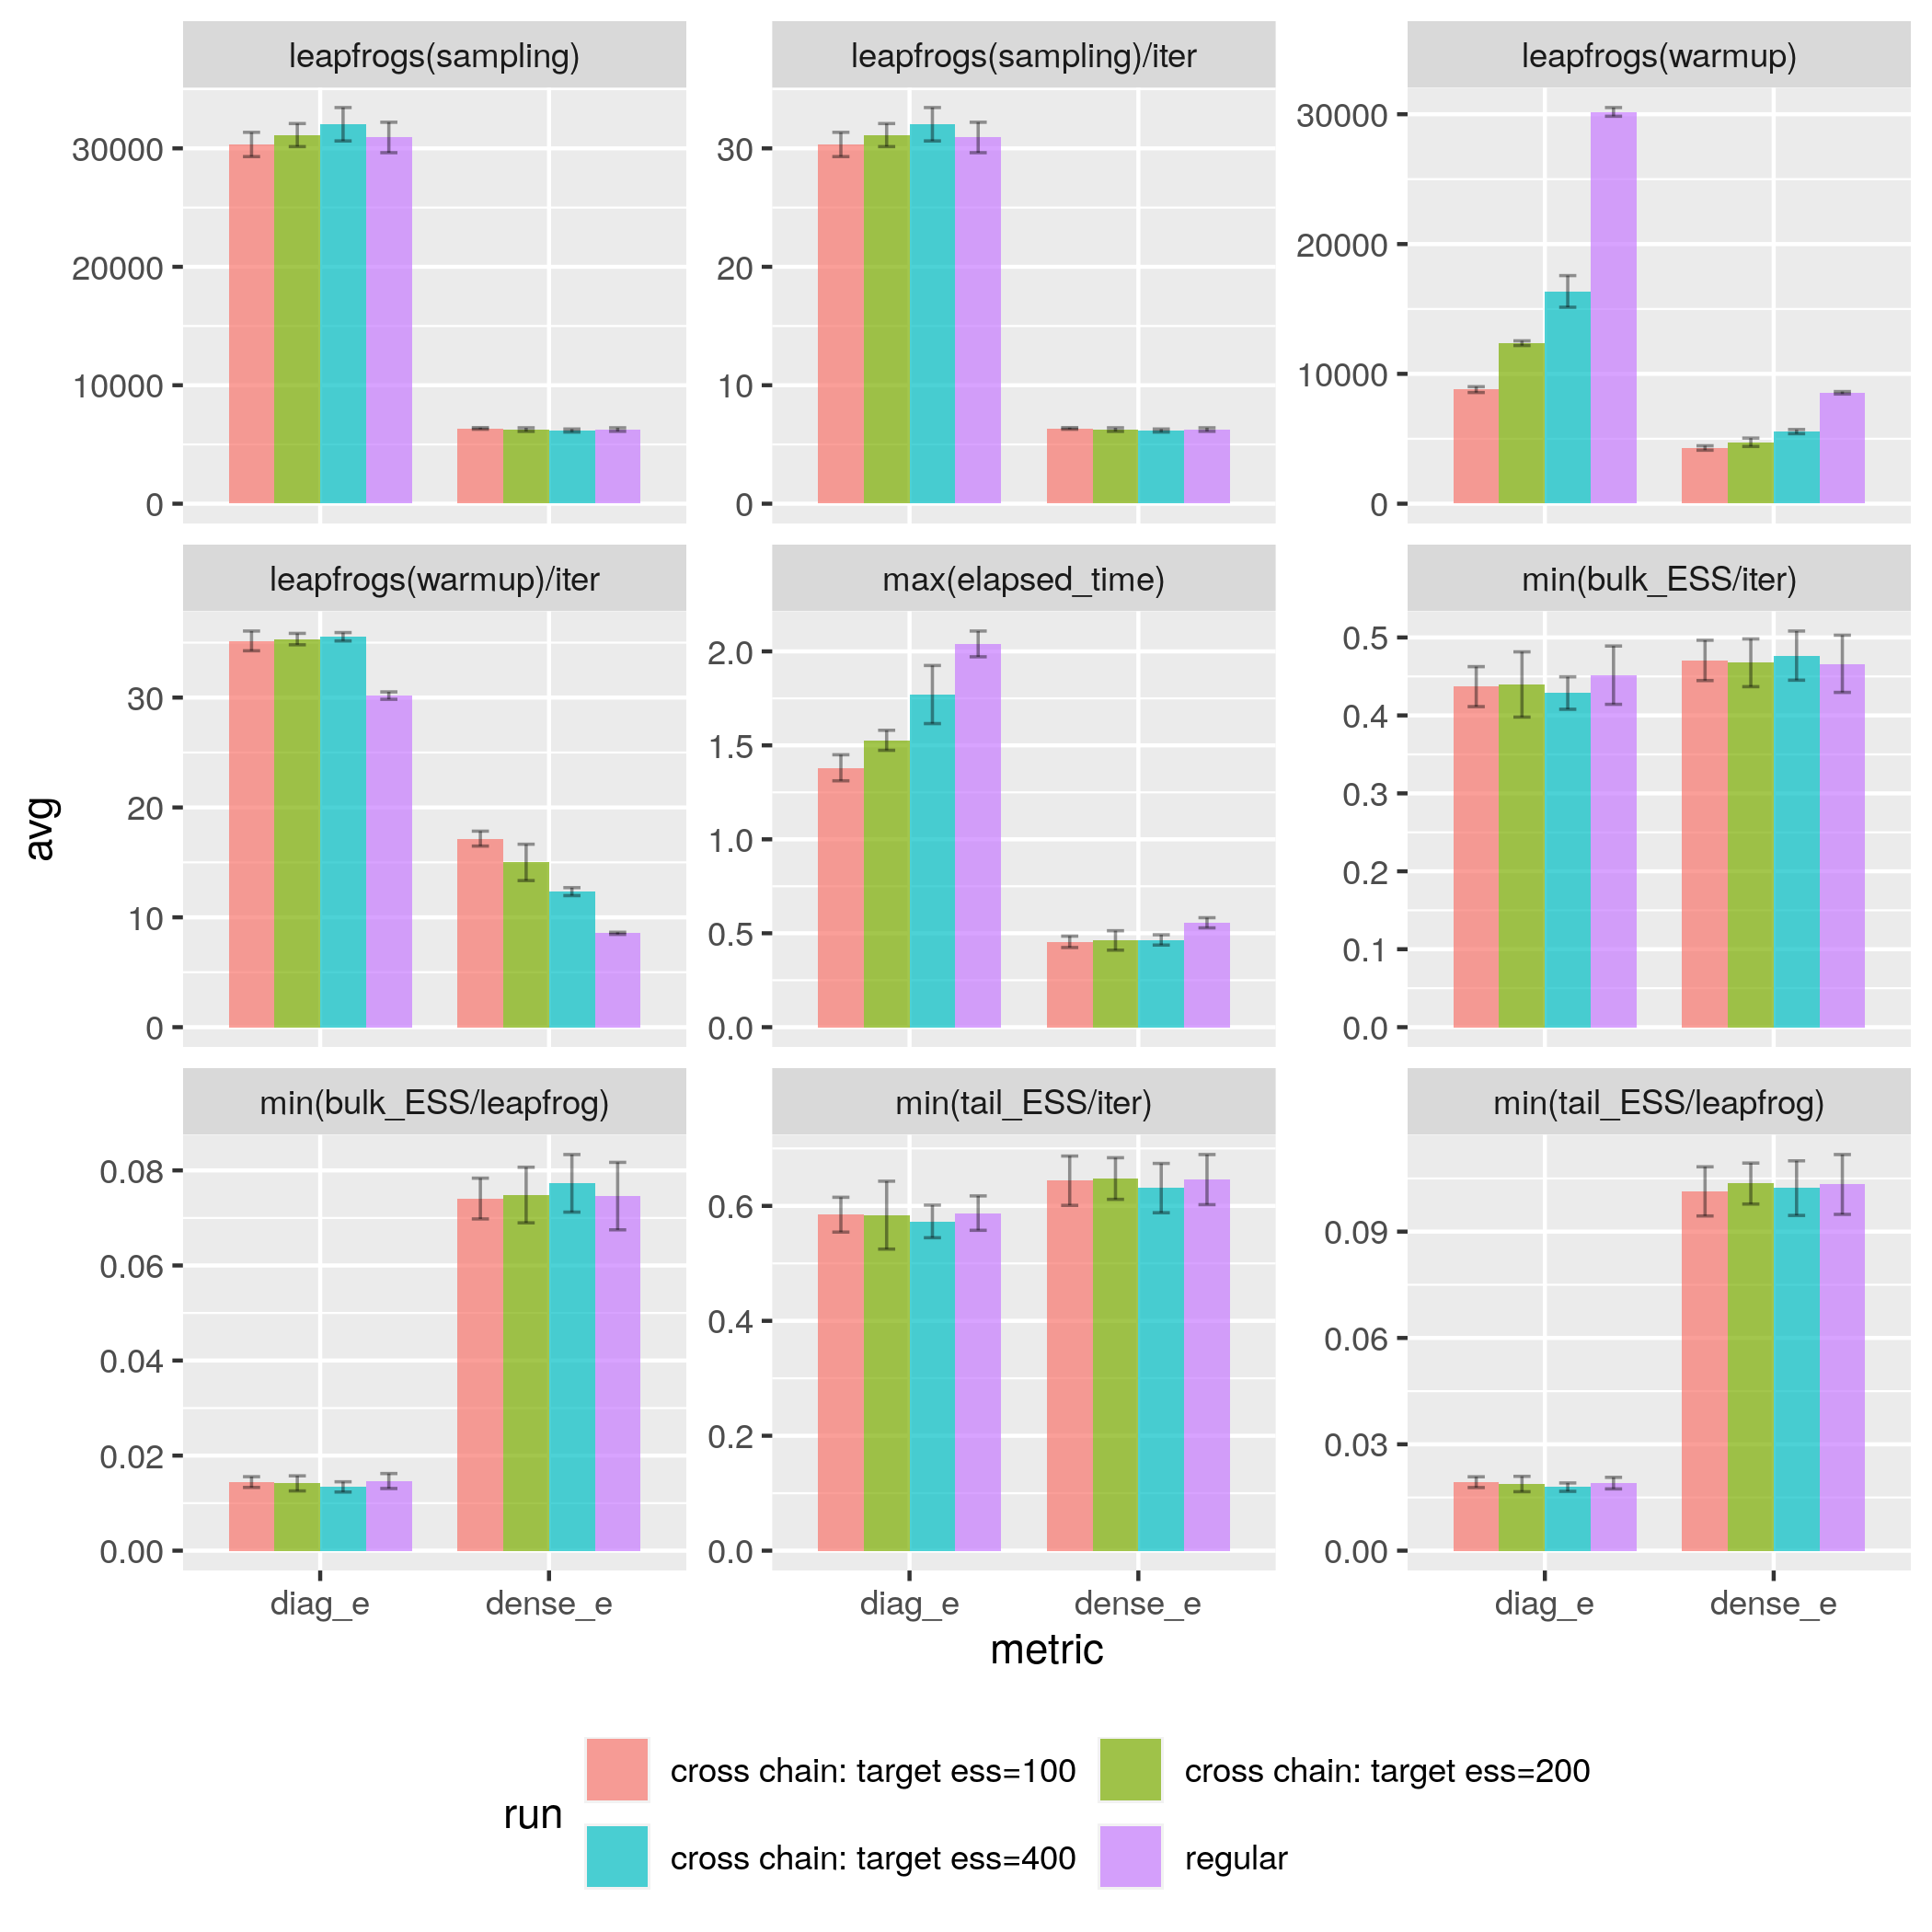
\includegraphics[width=\textwidth]{./figure/cross_chain_ess_effect_arK.png}
% \caption{Cross-chain warmup performance comparison: arK model}
% \end{figure}

% \begin{figure}[htbp]
% \centering
% 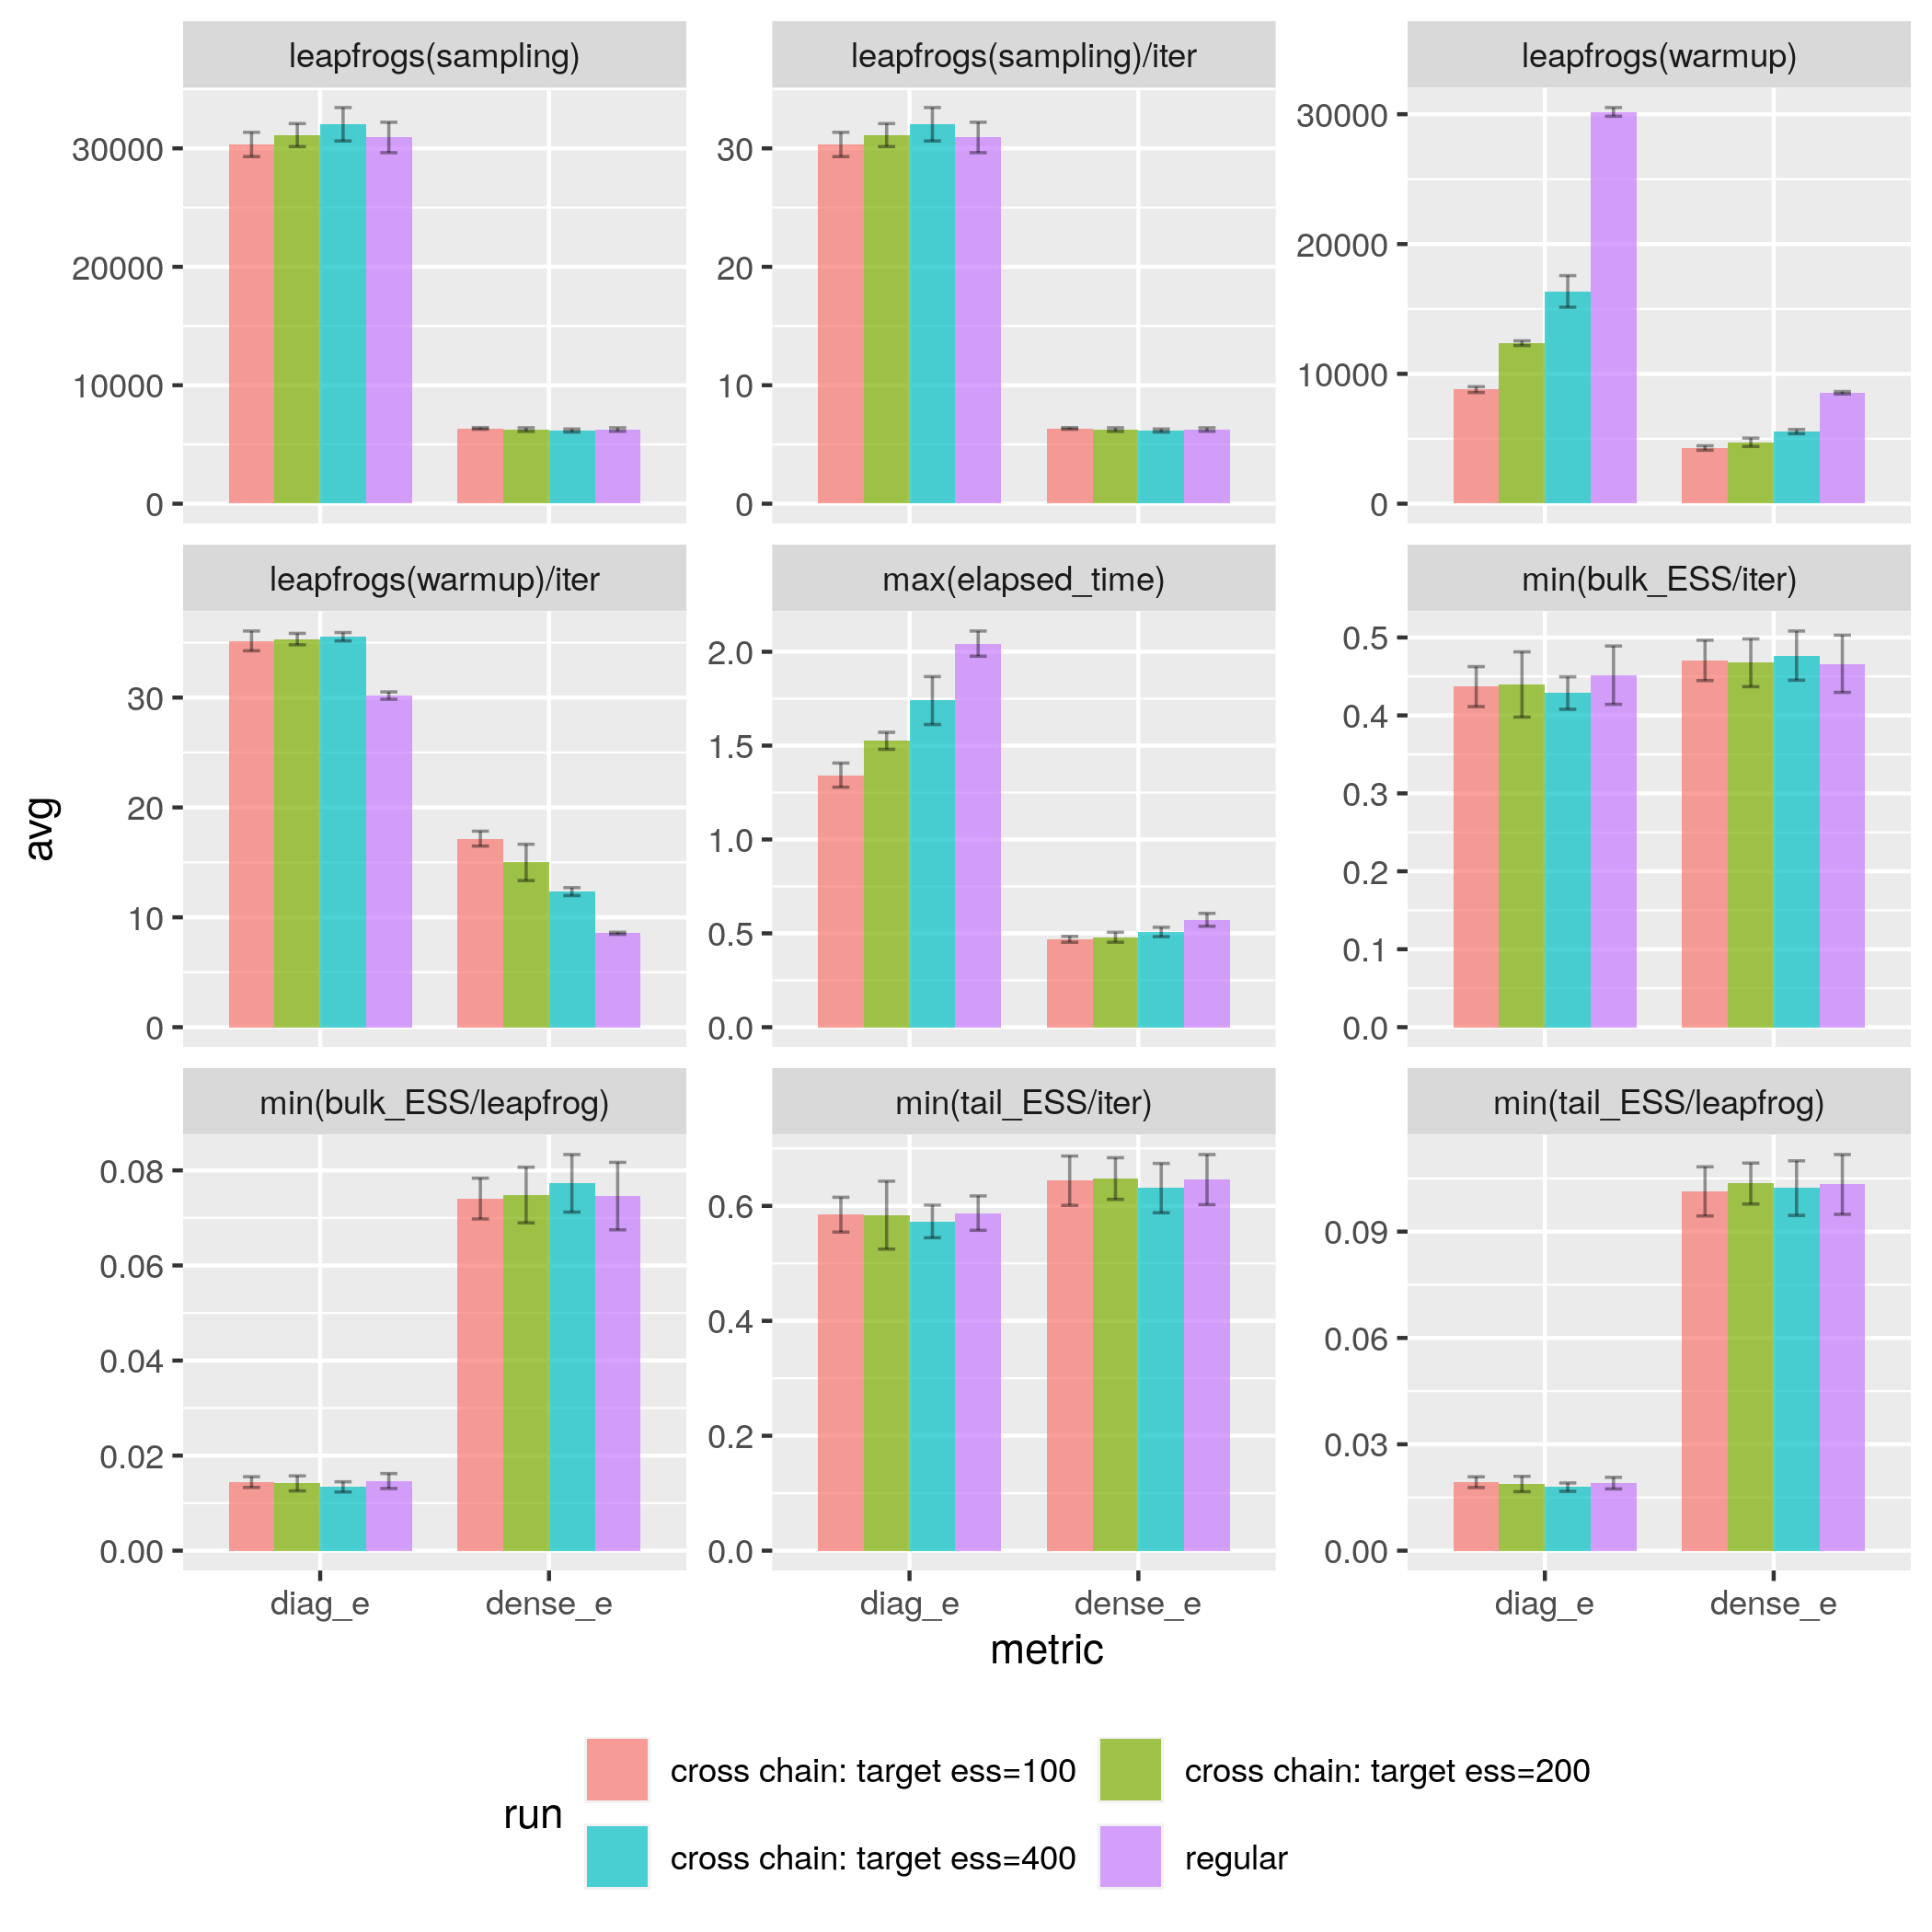
\includegraphics[width=\textwidth]{./figure/cross_chain_ess_effect_arK-arK.png}
% \caption{Cross-chain warmup performance comparison: arK-arK model}
% \end{figure}

% \begin{figure}[htbp]
% \centering
% 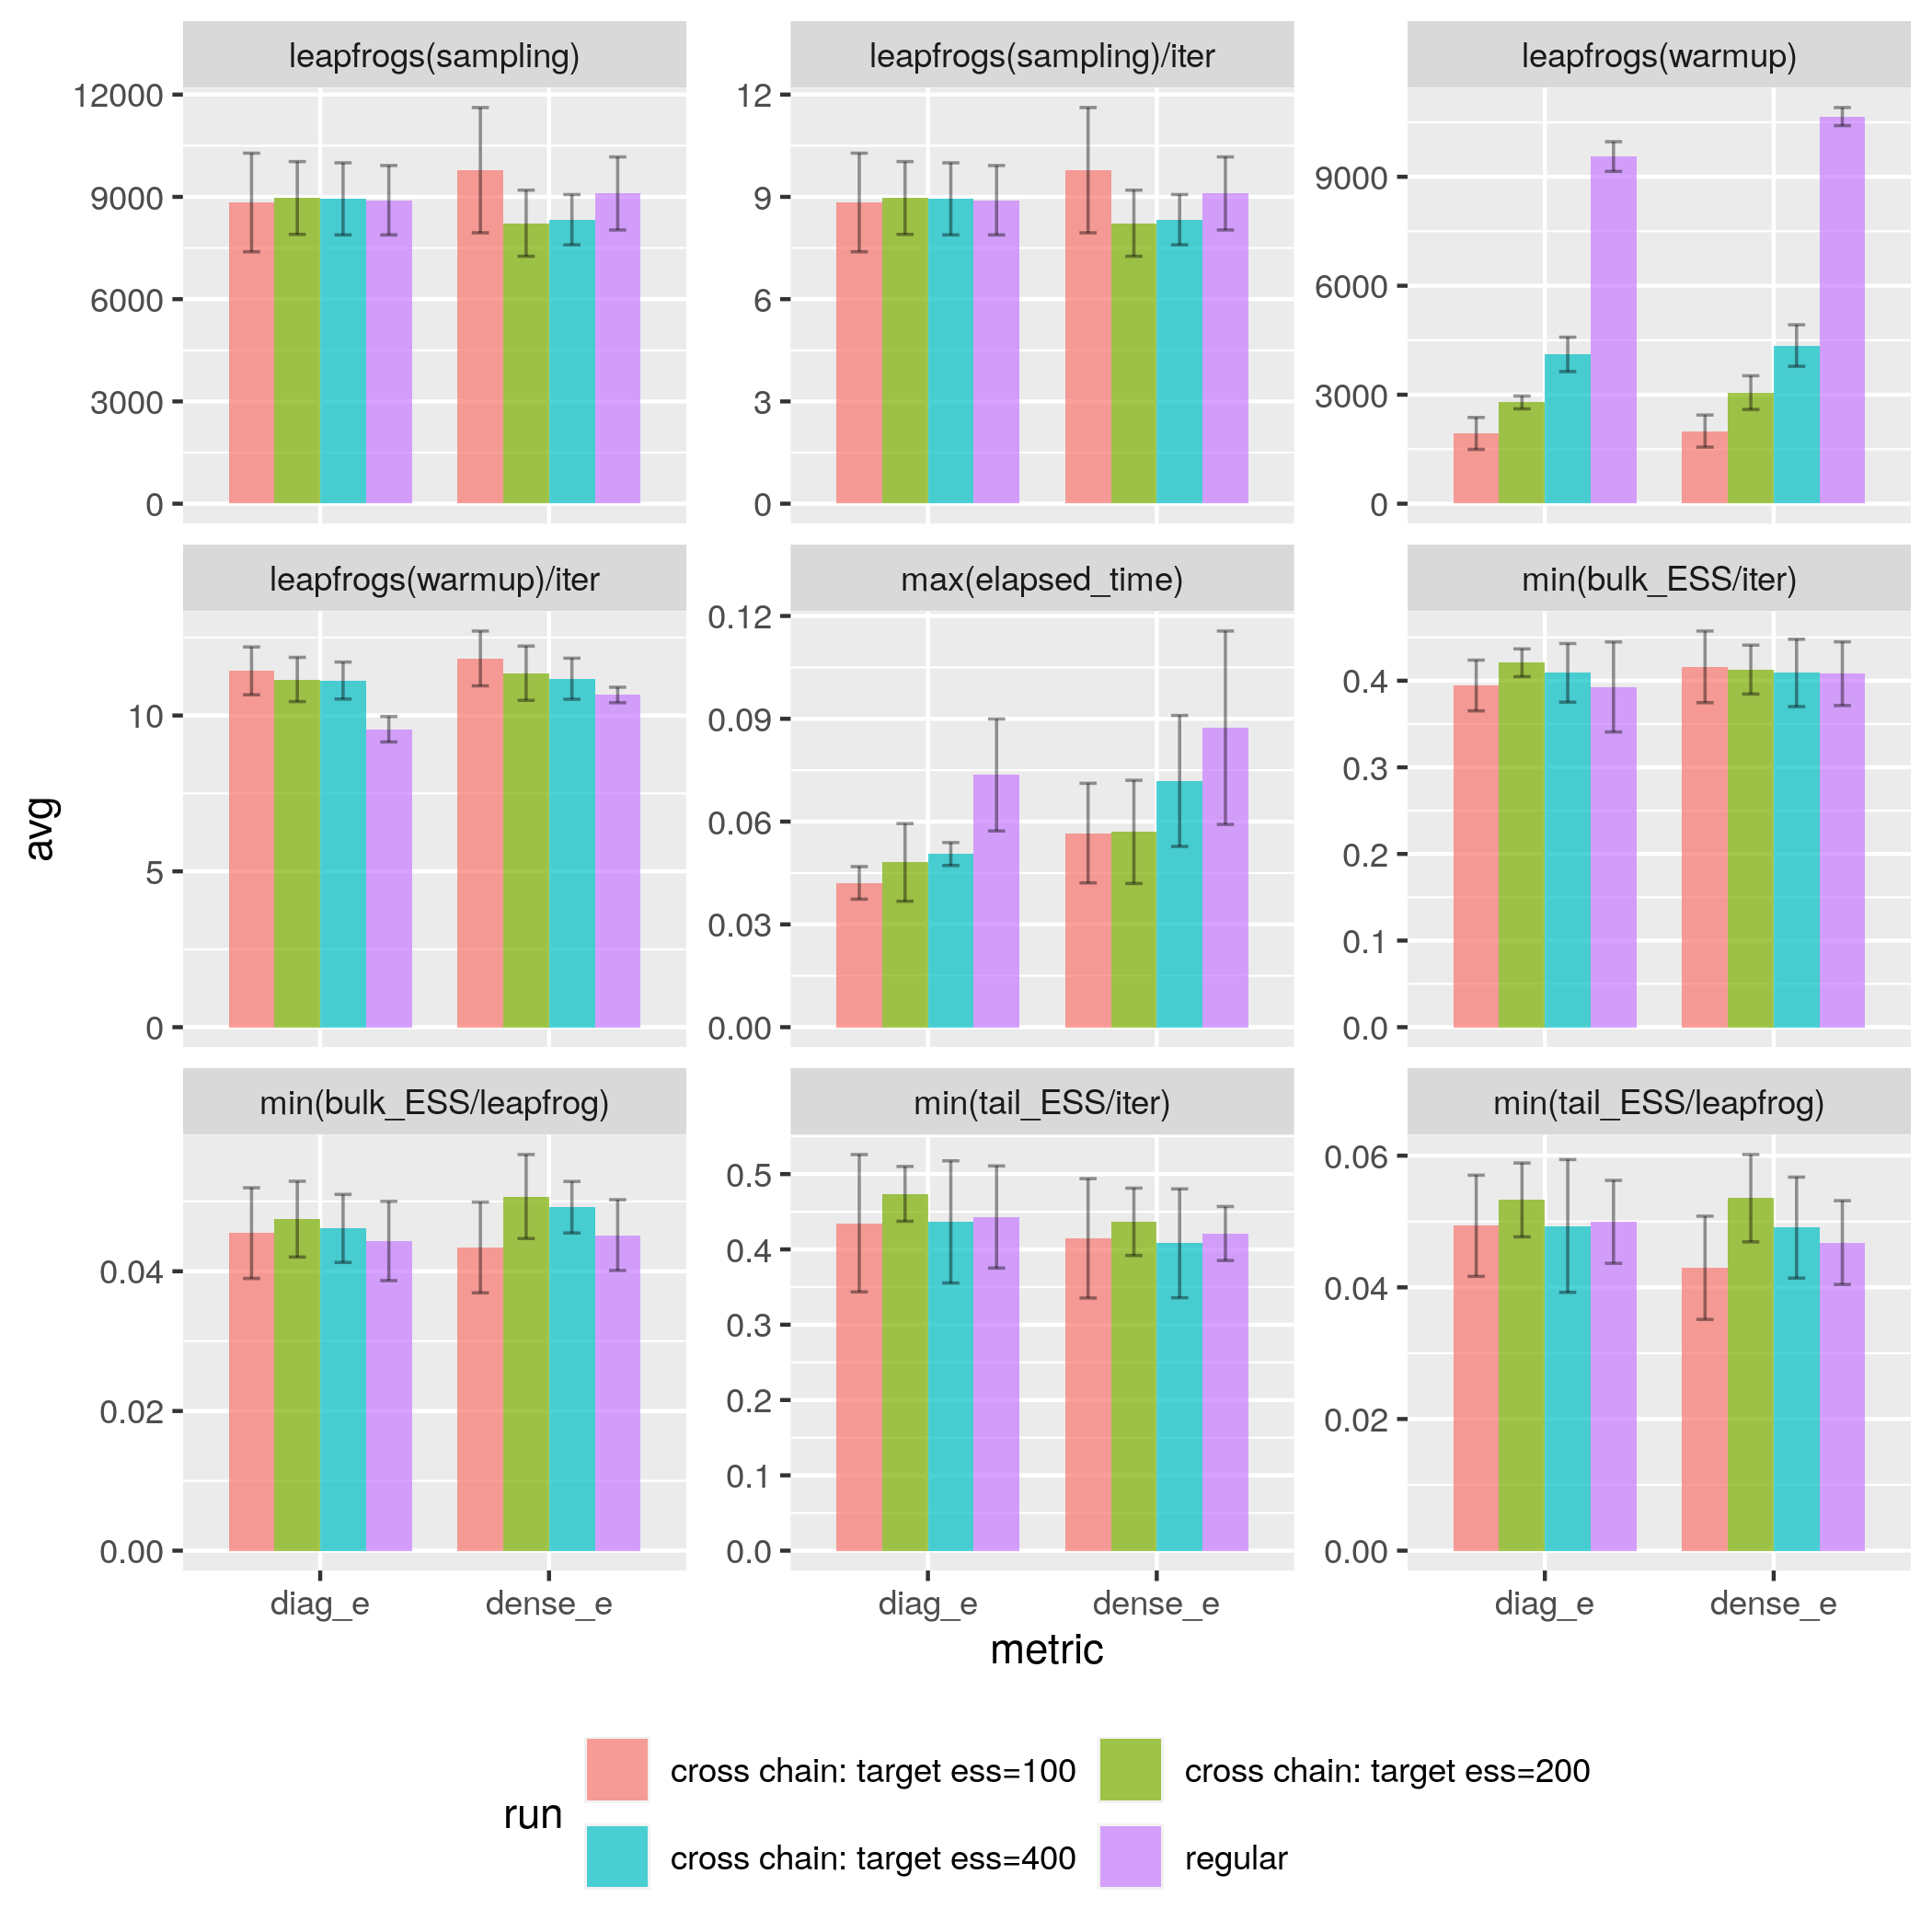
\includegraphics[width=\textwidth]{./figure/cross_chain_ess_effect_eight_schools.png}
% \caption{Cross-chain warmup performance comparison: eight schools model}
% \end{figure}

% \begin{figure}[htbp]
% \centering
% 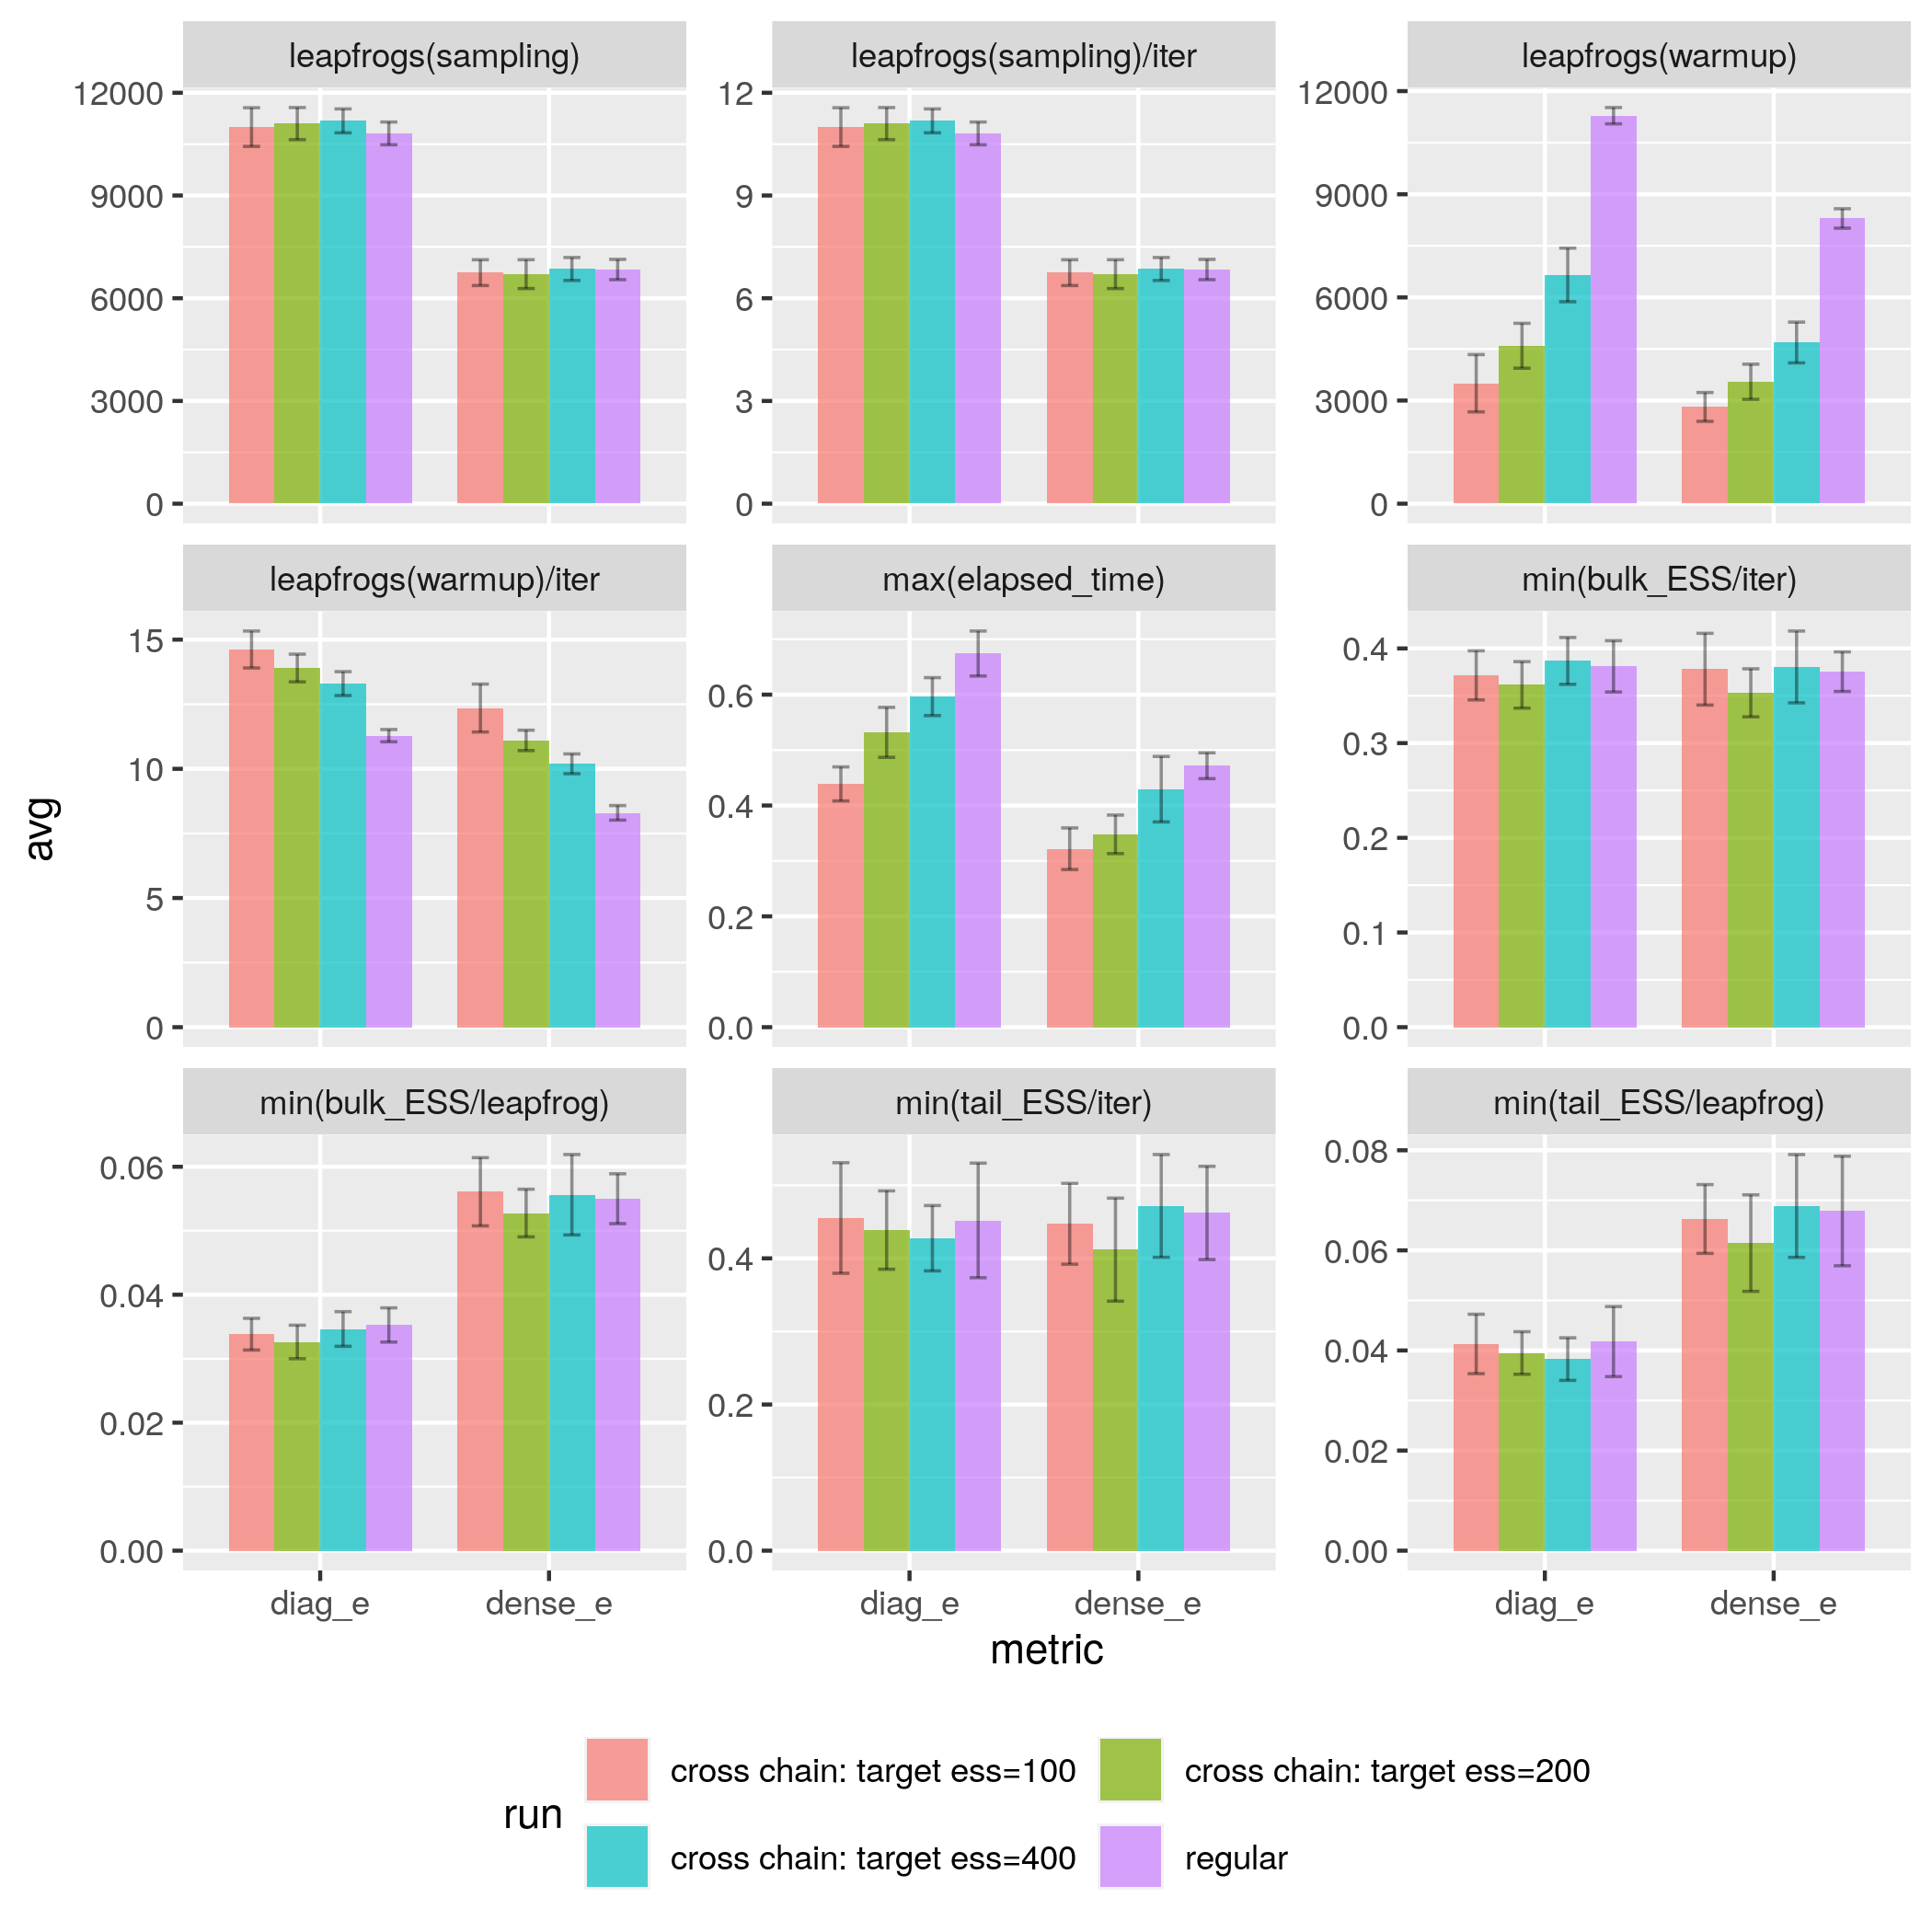
\includegraphics[width=\textwidth]{./figure/cross_chain_ess_effect_garch-garch11.png}
% \caption{Cross-chain warmup performance comparison: garch-garch11 model}
% \end{figure}

% \begin{figure}[htbp]
% \centering
% 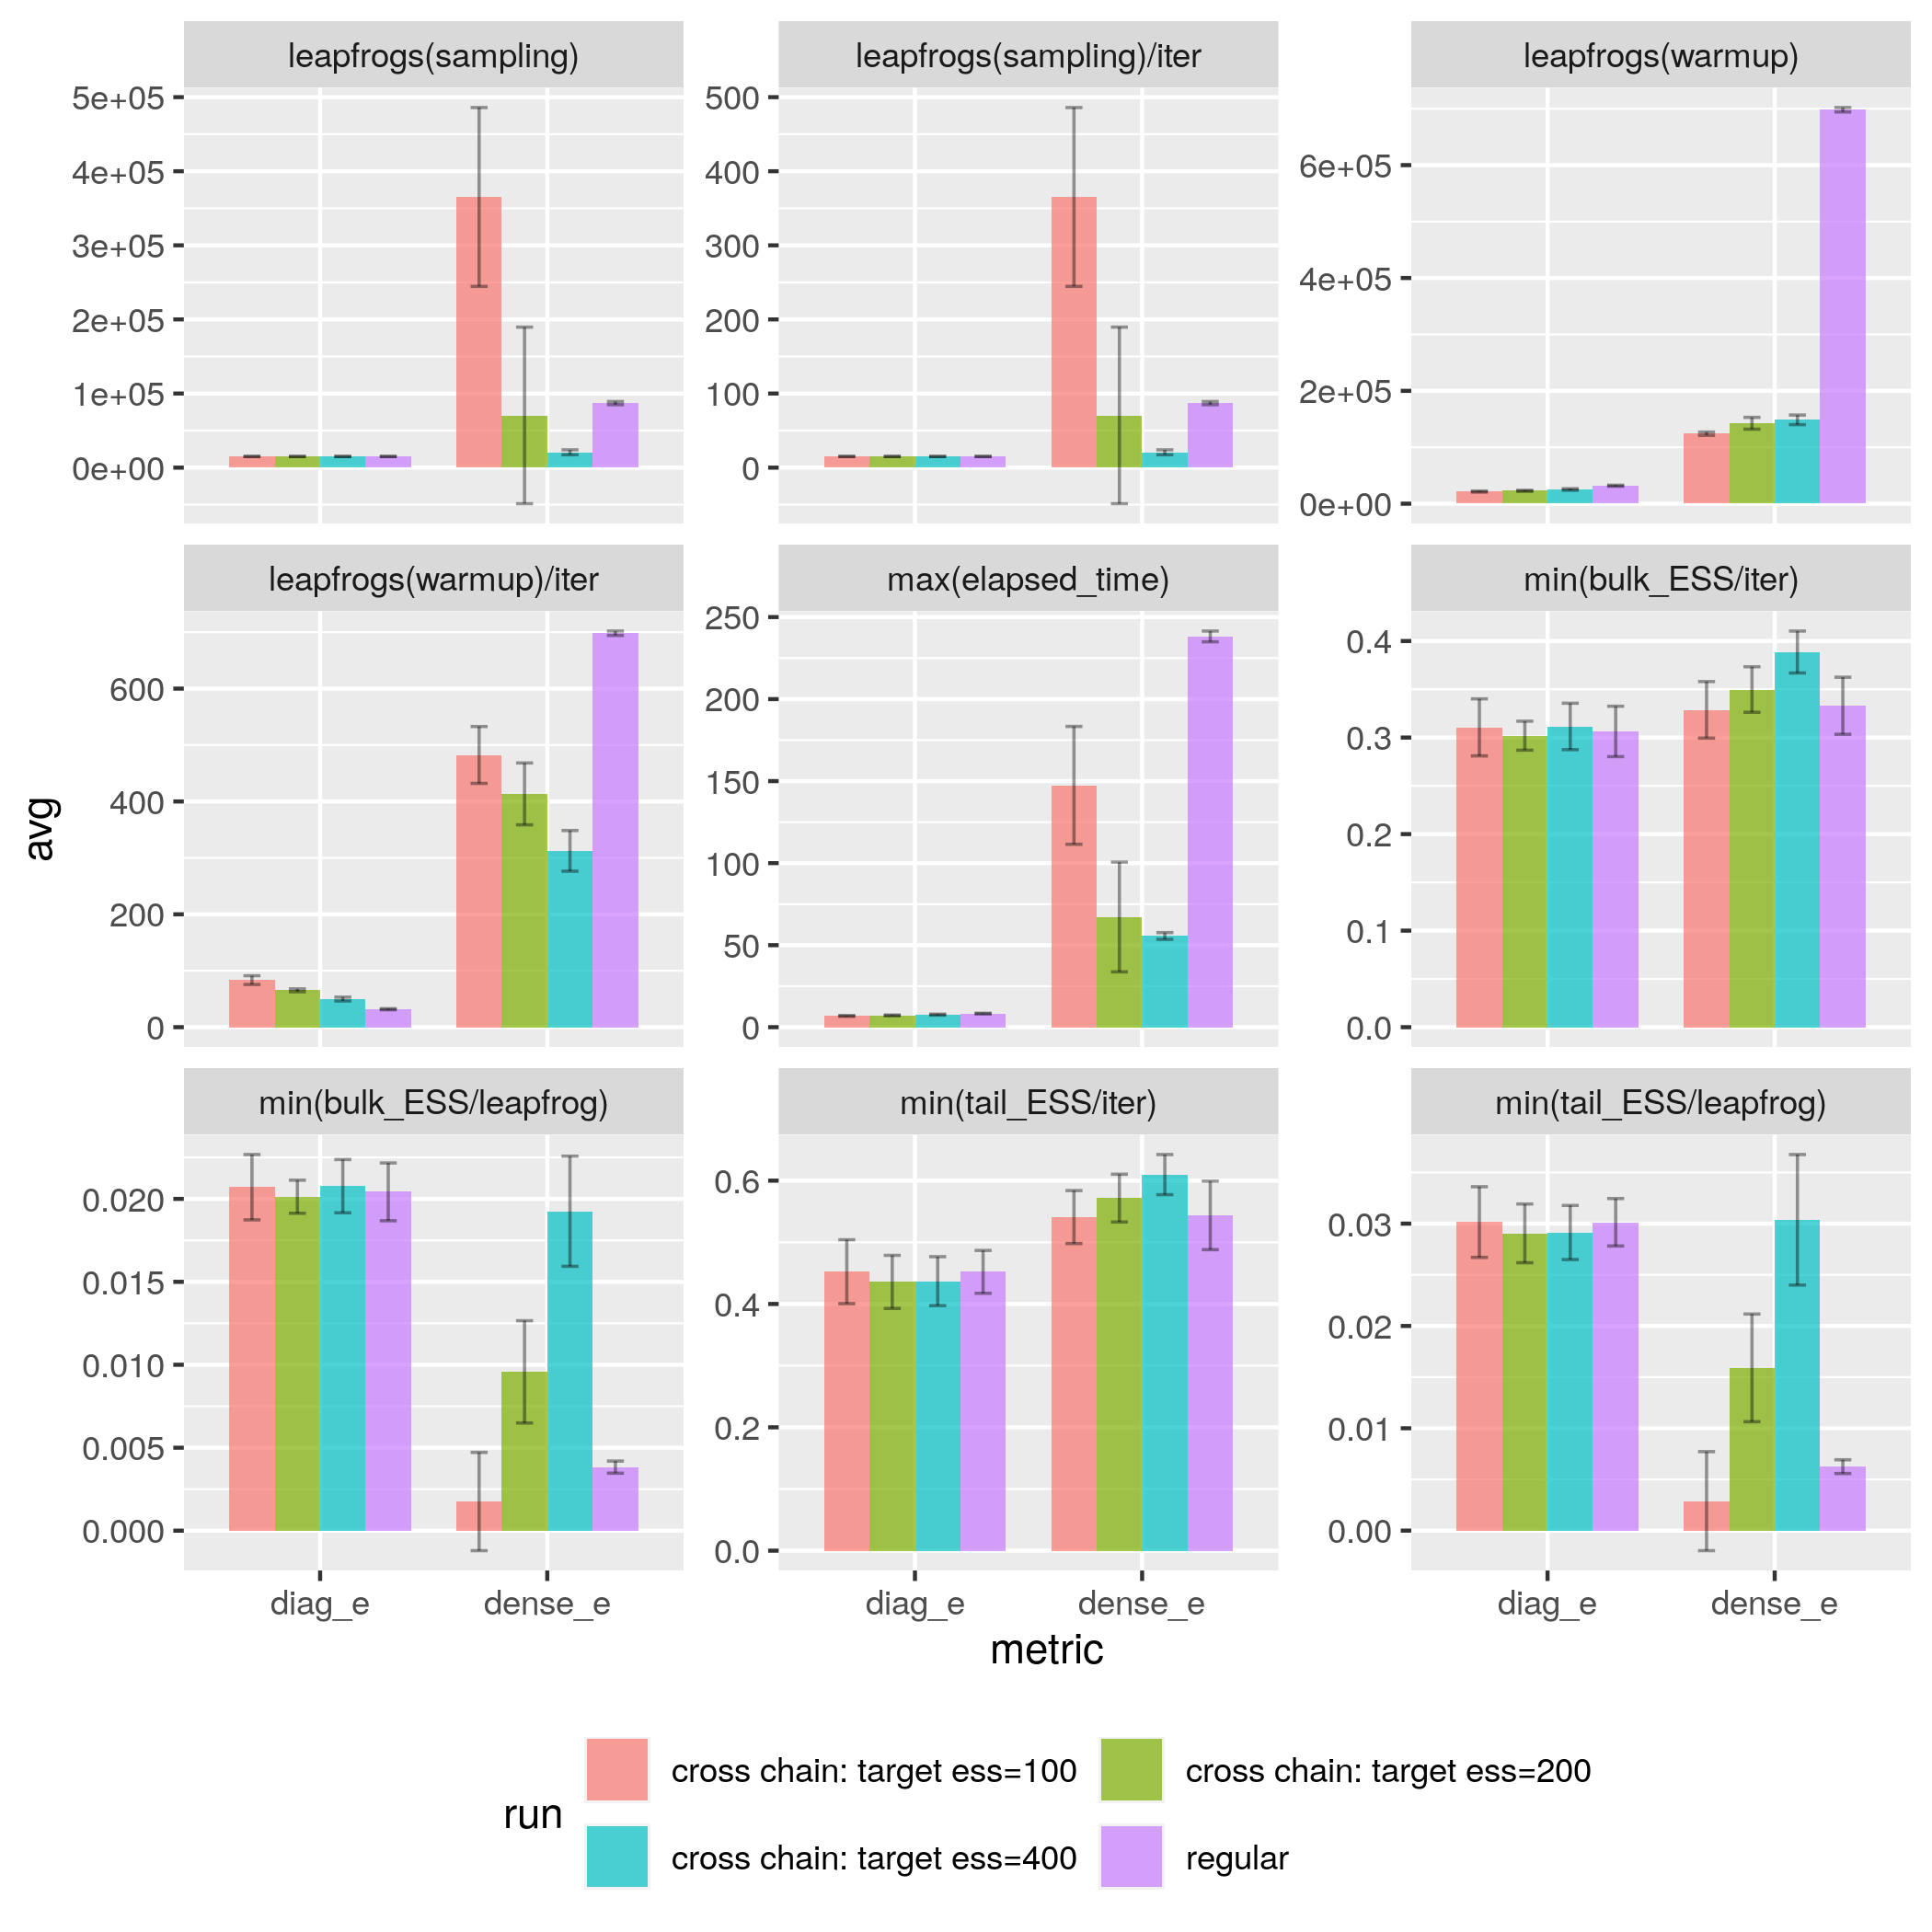
\includegraphics[width=\textwidth]{./figure/cross_chain_ess_effect_radon.png}
% \caption{Cross-chain warmup performance comparison: radon model}
% \end{figure}

% \begin{figure}[htbp]
% \centering
% 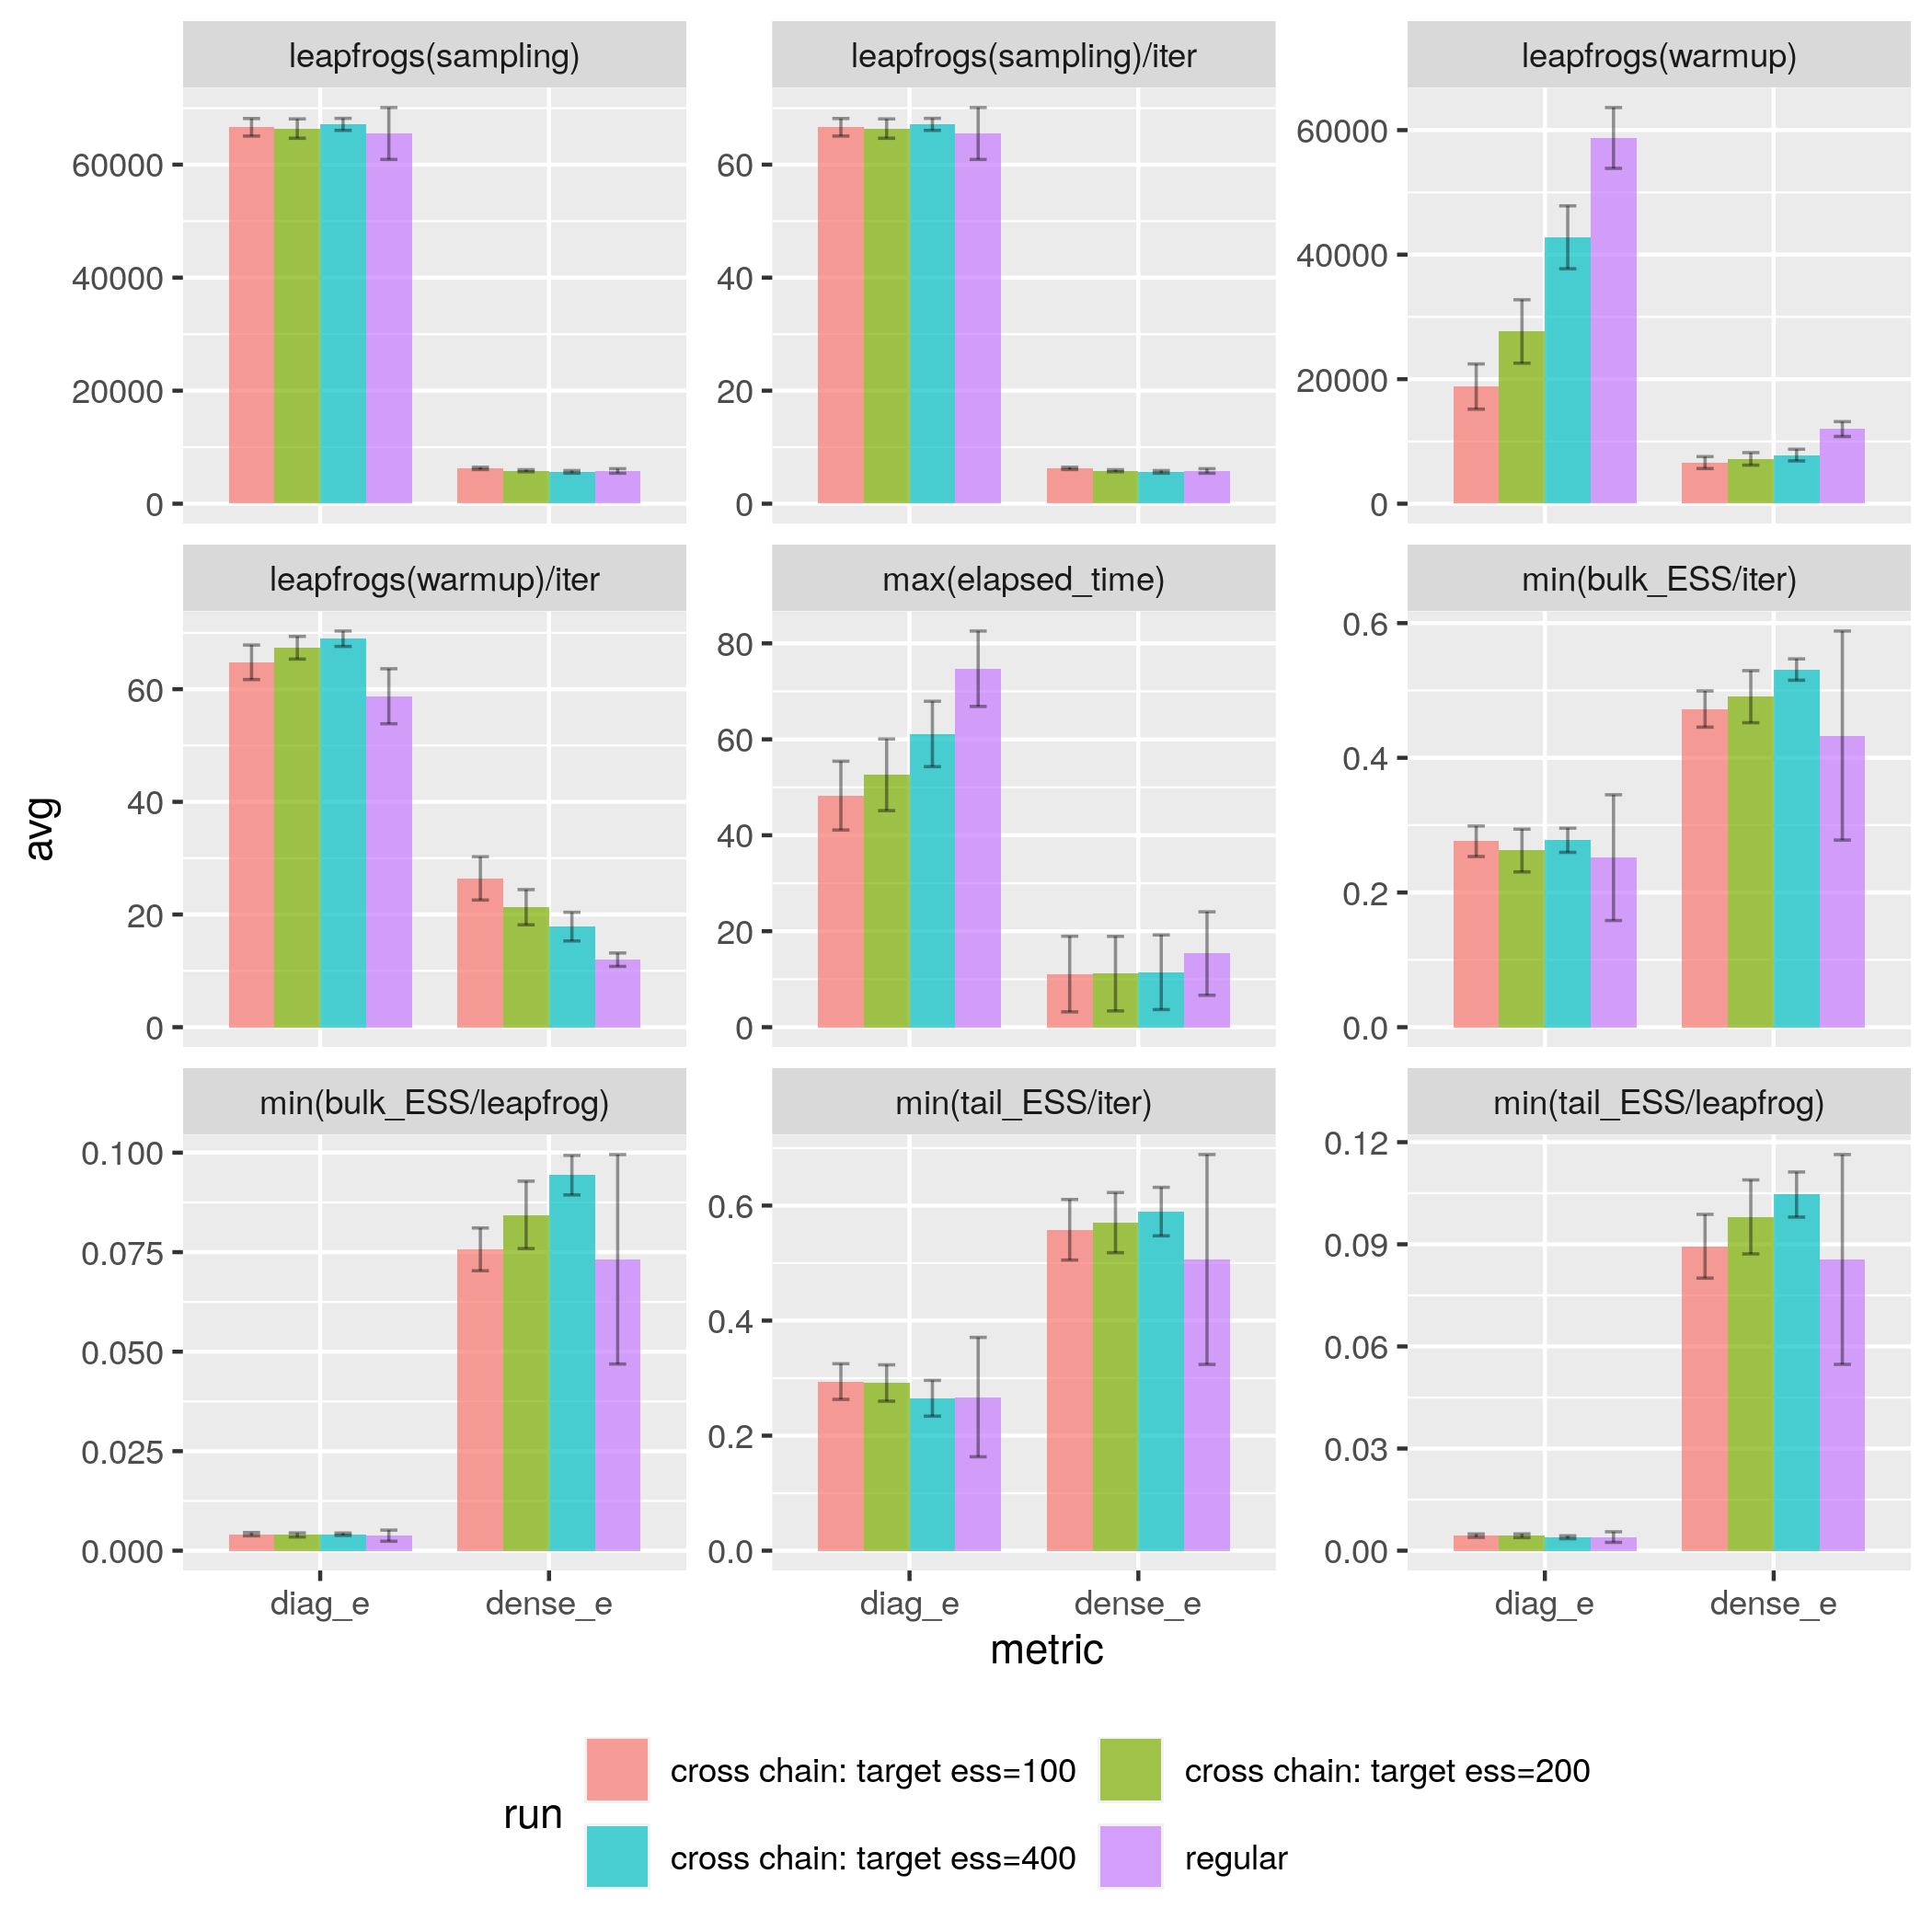
\includegraphics[width=\textwidth]{./figure/cross_chain_ess_effect_sir.png}
% \caption{Cross-chain warmup performance comparison: SIR model}
% \end{figure}

% \begin{figure}[htbp]
% \centering
% 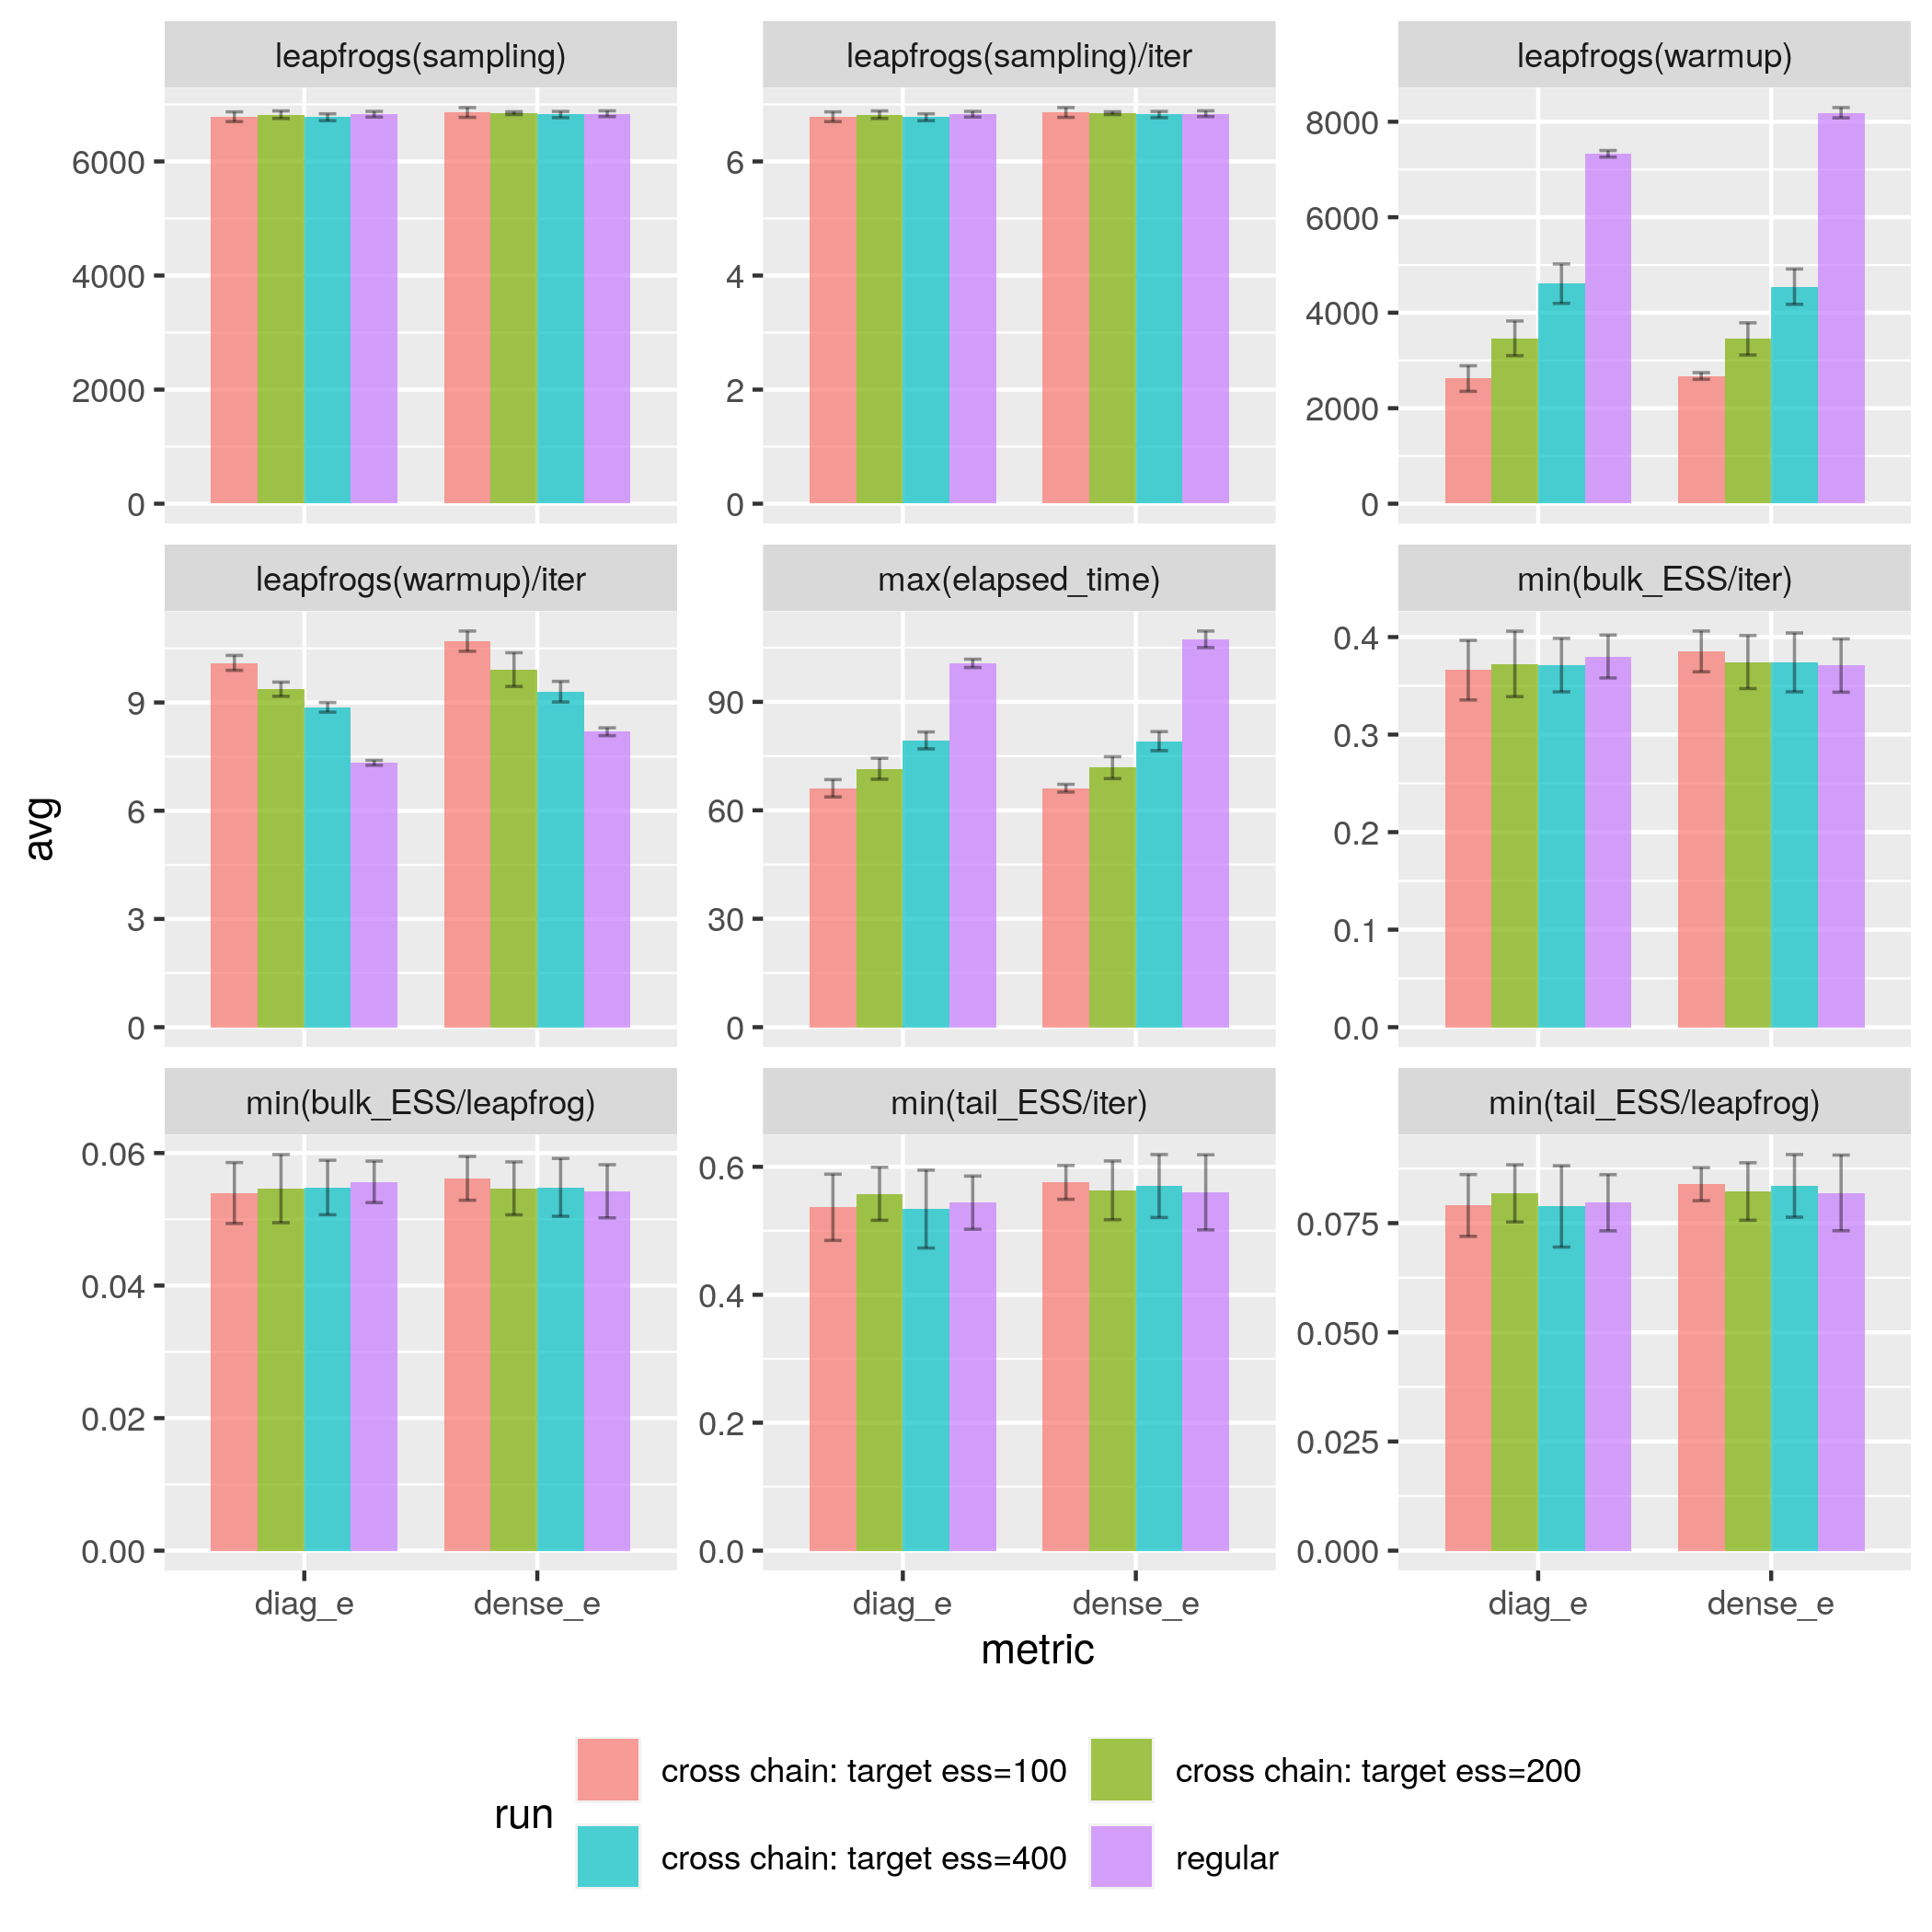
\includegraphics[width=\textwidth]{./figure/cross_chain_ess_effect_chem.png}
% \caption{Cross-chain warmup performance comparison: chemical reaction model}
% \end{figure}
}

% %----------------------------------------------------------------------------------------
% %	RESULTS 2
% %----------------------------------------------------------------------------------------

% \headerbox{Results 2}{name=results2,column=1,below=introduction,bottomaligned=conclusion}{ % This block's bottom aligns with the bottom of the conclusion block

% Donec faucibus purus at tortor egestas eu fermentum dolor facilisis. Maecenas tempor dui eu neque fringilla rutrum. Mauris \emph{lobortis} nisl accumsan.

% \begin{center}
% \begin{tabular}{l l l}
% \toprule
% \textbf{Treatments} & \textbf{Response 1} & \textbf{Response 2}\\
% \midrule
% Treatment 1 & 0.0003262 & 0.562 \\
% Treatment 2 & 0.0015681 & 0.910 \\
% Treatment 3 & 0.0009271 & 0.296 \\
% \bottomrule
% \end{tabular}
% \captionof{table}{Table caption}
% \end{center}

% Nulla ut porttitor enim. Suspendisse venenatis dui eget eros gravida tempor. Mauris feugiat elit et augue placerat ultrices. Morbi accumsan enim nec tortor consectetur non commodo.

% \begin{center}
% \begin{tabular}{l l l}
% \toprule
% \textbf{Treatments} & \textbf{Response 1} & \textbf{Response 2}\\
% \midrule
% Treatment 1 & 0.0003262 & 0.562 \\
% Treatment 2 & 0.0015681 & 0.910 \\
% Treatment 3 & 0.0009271 & 0.296 \\
% \bottomrule
% \end{tabular}
% \captionof{table}{Table caption}
% \end{center}
% }

%----------------------------------------------------------------------------------------

\end{poster}

\end{document}
